\documentclass[draft]{agujournal2019}
\usepackage{url} %this package should fix any errors with URLs in refs.
\usepackage{lineno}
\usepackage[inline]{trackchanges} %for better track changes. finalnew option will compile document with changes incorporated.
\usepackage{soul}
\linenumbers

% --- My additions
\usepackage{amsmath}
\usepackage{amssymb}
\usepackage{mathtools} % for coloneqq
\usepackage{todonotes}
\usepackage{overpic}
\usepackage{rnn}
\usepackage[capitalise,noabbrev]{cleveref}

\crefname{appendix}{}{} % gets rid of Appendix Appendix A

\newcommand{\red}[1]{\textcolor{red}{#1}}
\newcommand{\blue}[1]{\textcolor{blue}{#1}}

\newcommand{\citep}{\cite}
\newcommand{\citet}{\citeA}

%%%%%%%
% As of 2018 we recommend use of the TrackChanges package to mark revisions.
% The trackchanges package adds five new LaTeX commands:
%
%  \note[editor]{The note}
%  \annote[editor]{Text to annotate}{The note}
%  \add[editor]{Text to add}
%  \remove[editor]{Text to remove}
%  \change[editor]{Text to remove}{Text to add}
%
% complete documentation is here: http://trackchanges.sourceforge.net/
%%%%%%%

\draftfalse

\journalname{Journal of Advances in Modeling Earth Systems (JAMES)}


\begin{document}

\title{Recurrent Neural Network Emulation of Turbulent Geophysical Fluids}
% Considered "high resolution GFD", but SQG is not necessarily high resolution, just well-resolved turbulence.
% This is clearly TBD...

%% ------------------------------------------------------------------------ %%
%
%  AUTHORS AND AFFILIATIONS
%
%% ------------------------------------------------------------------------ %%

% Example: \authors{A. B. Author\affil{1}\thanks{Current address, Antartica}, B. C. Author\affil{2,3}, and D. E.
% Author\affil{3,4}\thanks{Also funded by Monsanto.}}

\authors{(To be ordered)
Timothy A. Smith\affil{1,2},
Stephen G. Penny\affil{1,3},
Jason A. Platt\affil{4},
Tse-Chun Chen\affil{1,2}
}
\affiliation{1}{Cooperative Institute for Research in Environmental Sciences
    (CIRES) at the University of Colorado Boulder, Boulder, CO, USA
}
\affiliation{2}{Physical Sciences Laboratory (PSL), National Oceanic and
    Atmospheric Administration (NOAA), Boulder, CO, USA
}
\affiliation{3}{Sofar Ocean}
\affiliation{4}{UCSD}

%% Corresponding Author:
\correspondingauthor{Timothy A. Smith}{tim.smith@noaa.gov}

%% Keypoints, final entry on title page.

% This is a work in progress, just trying to focus my thoughts.
\begin{keypoints}
    \item Implement recurrent neural networks for predicting turbulent geophysical flows
    \item In QG dynamics, the RNNs capture large scale features and perform .. compared to baseline metrics
    \item Application to high resolution reanalysis output suggests
\end{keypoints}

%% ------------------------------------------------------------------------ %%
%
%  ABSTRACT and PLAIN LANGUAGE SUMMARY
%
%% ------------------------------------------------------------------------ %%

\begin{abstract}
[ enter your Abstract here ]
\end{abstract}

\section*{Plain Language Summary}
[ enter your Plain Language Summary here or delete this section]


%% ------------------------------------------------------------------------ %%
%
%  TEXT
%
%% ------------------------------------------------------------------------ %%

\section{Introduction}
\label{sec:intro}

% Climate and weather models are expensive, and we really want ensembles
Weather and climate prediction requires the integration of a computational
model derived from the fundamental equations of motion and initialized
with an estimate of the present-day system state (e.g., temperature, wind speeds,
etc.).
Due to the high computational cost of the physical model, prediction systems
typically require suboptimal tradeoffs.
On one hand, it is desirable to increase the credibility of the underlying
numerical model as much as possible,
for instance by increasing model grid resolution
\citep <e.g.,>[]{hewitt_impact_2016}
or by explicitly
simulating as many coupled components (e.g., atmosphere, land, ocean, ice) as
possible \citep <e.g.,>[]{penny_coupled_2017}.
On the other hand, knowledge of the model initial conditions is imperfect and
the governing equations will always contain necessary, inexact approximations of
reality.
As a result, prediction systems employ
statistical methods like ensemble based forecasting in order to represent this
uncertainty.
Producing an ensemble with statistical significance
requires integrating the underlying numerical model many times; usually
$\mathcal{O}(10-100)$ in practice, but ideally $>1,000$
\citep{evensen_data_2022}.
Therefore, the resulting computational costs require practitioners to trade between the
fidelity of the numerical model and credibility of the statistical method.

% Surrogate modeling an encouraging path, and with increased computing power,
% ML, NNs ...
An ongoing area of research that aims to enable statistical forecasting subject
to the dynamics of an expensive numerical model is \textit{surrogate modeling}.
The general approach relies on using a model that represents or ``emulates'' the
dynamics of the original numerical model ``accurately enough'' for the given
application, while being computationally inexpensive to evaluate.
Historically, surrogate models have been developed with techniques like
Linear Inverse Models
\citep <e.g.,
principal oscillation or interaction patterns;>[]{hasselmann_pips_1988,penland_random_1989, moore_linear_2022},
kriging \citep{cressie_statistics_1993},
more general projection based reduced order modeling \citep{bui-thanh_model_2008},
or
polynomial chaos techniques \citep{najm_uncertainty_2009},
to name only a few.
More recently, advances in computing power and the explosion of freely available data
%and more widespread usage of General Purpose Graphics Processing Units (GPGPUs)
has encouraged the exploration of more expensive machine learning methods like
neural networks for the emulation task \citep{schultz_can_2021}.
A number of data-driven, neural network architectures have been developed to
generate surrogate models for weather forecasting and climate projection
applications.
Some examples include models based on
feed forward neural networks
\citep{dueben_challenges_2018},
convolutional neural networks
\citep <CNNs;>[]{scher_toward_2018,scher_weather_2019,rasp_data-driven_2021,weyn_can_2019,weyn_improving_2020,weyn_sub-seasonal_2021},
recurrent neural networks
\citep <RNNs;>[]{arcomano_machine_2020,chen_predicting_2021,nadiga_reservoir_2021},
graph neural networks \citep{keisler_forecasting_2022,lam_graphcast_2022},
Fourier neural operators \citep{pathak_fourcastnet_2022},
and encoder-transformer-decoder networks
\citep{bi_pangu-weather_2022}.

A significant advancement in surrogate modeling for weather and climate prediction
has been the rapid increase in horizontal grid resolution.
To the best of our knowledge, the current highest resolution neural network
emulators for
global atmospheric dynamics is $\sim0.25^\circ$ ($\sim$31~km)
\citep{pathak_fourcastnet_2022,bi_pangu-weather_2022,lam_graphcast_2022},
which is the same
resolution as the ERA5 Reanalysis \citep{hersbach_era5_2020} used for
training.
At this resolution, General Circulation Models (GCMs) of the atmosphere are
capable of expliciting capturing important small scale processes like
interactions with mountainous topography.
However, it is not yet clear that neural networks are able to
represent the same dynamical processes as a GCM at identical grid resolution.
Instead, based on our own experimentation, we hypothesize that without careful
architectural modifications, neural network emulators will effectively operate at a coarser
resolution than the grid scale would otherwise indicate.

\begin{figure}
    \centering
    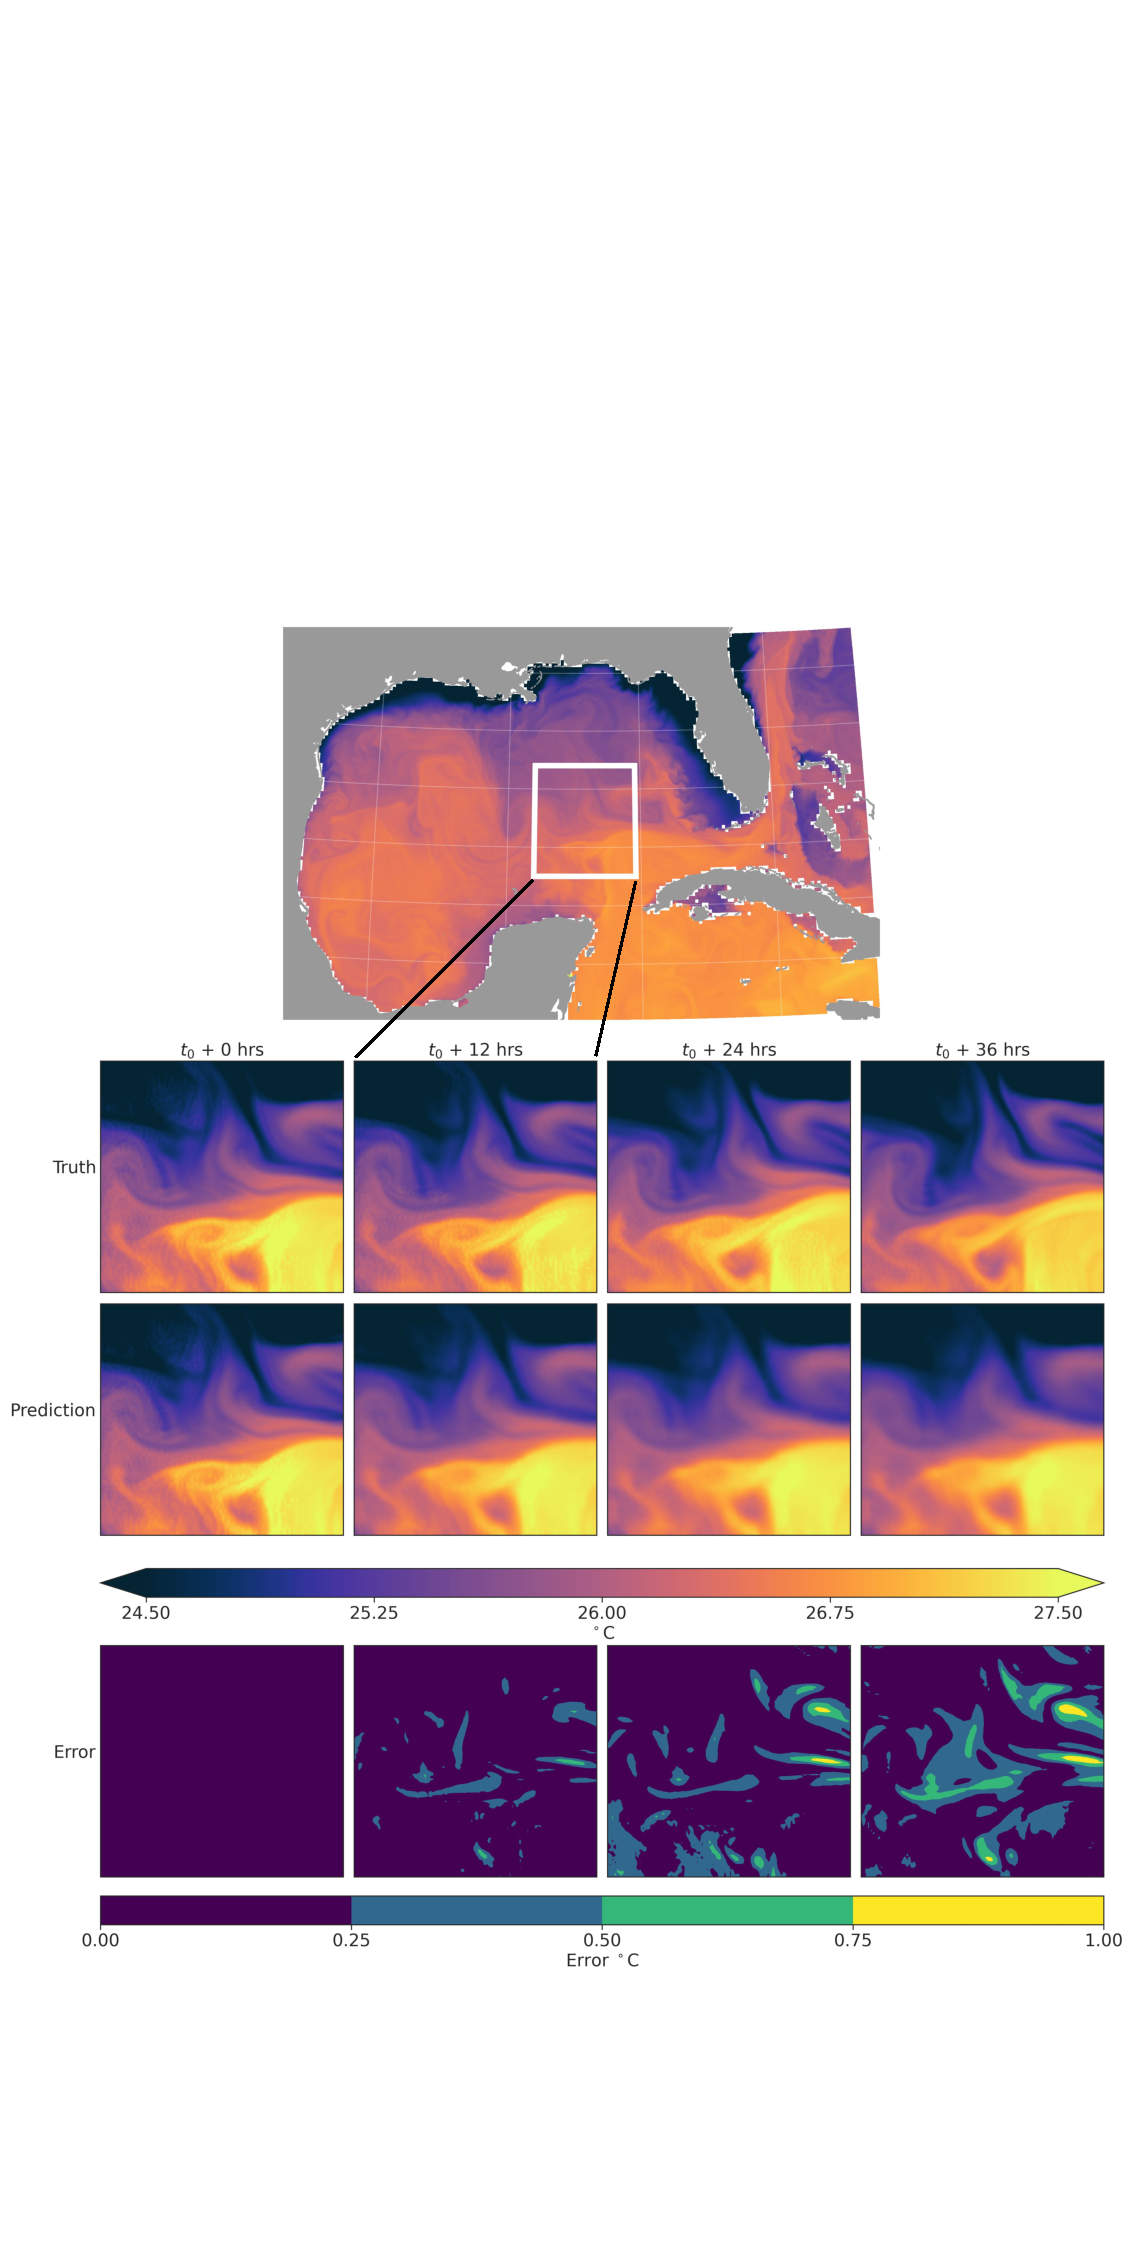
\includegraphics[width=.8\textwidth]{../figures/rc_gom_sst.pdf}
    \caption{A sample prediction of sea surface temperatures in the Gulf of Mexico at 1/25$^\circ$
        horizontal resolution.
        The upper row (Truth) shows the evolution of unseen test data from the
        Navy/HYCOM reanalysis product, and the middle row shows a prediction
        from the Echo State Network architecture described in
        \cref{subsec:rc}.
        The bottom row (Error) shows the absolute value of the difference between the two.
        See \cref{sec:gom} for a description of the dataset.
    }
    \label{fig:gom_sst}
\end{figure}

To make the discussion concrete, we present a sample prediction from our own surrogate model
in \cref{fig:gom_sst}.
The panels show the time evolution of Sea Surface
Temperature (SST) in the Gulf of Mexico at 1/25$^\circ$ horizontal resolution,
using data from a Navy/HYCOM, 3D-Var-based reanalysis product
as ``Truth'' (upper row; see \cref{sec:gom} for data details).
We generate the prediction (middle row) with an RNN architecture
described more fully in \cref{subsec:rc}.
Generally speaking, the RNN captures the largest scales of the SST pattern over
a 36~hour window.
However, as time progresses, the SST pattern becomes overly smooth.
The RNN is
unable to capture the spatial details that are well resolved in the reanalysis
dataset, with the largest errors evolving along sharp SST fronts.
We note that a similar smoothing behavior can be observed in other neural
network based emulators, see for example
\citep<>[Figure 1]{bi_pangu-weather_2022},
\citep<>[Figure 4c \& 4d]{pathak_fourcastnet_2022},
\citep<>[Figure 5]{keisler_forecasting_2022}


There are a number of reasons that could cause this smoothing behavior to manifest in the
predictions.
Our primary goal is to explore at least one reason why this occurs
and explore an optimization based technique to mitigate its effects.
%in order to understand what spatial scales can reliably be resolved.
We note that our example in \cref{fig:gom_sst} and many existing emulators use
reanalysis datasets as training data
\citep<e.g.>[]{lam_graphcast_2022,bi_pangu-weather_2022,pathak_fourcastnet_2022,keisler_forecasting_2022,weyn_sub-seasonal_2021,arcomano_machine_2020}.
There are many excellent reasons to use reanalysis products as training
data; namely they are constrained to observational data.
However, we contend that there are imperfections with reanalysis datasets that
need to be understood in order to be used in data-driven methods.
For instance, reanalyses typically contain jumps in the state vector at the
start of each data assimilation window, and due to the massive size of the data,
they are typically only available at time intervals longer than the timestep
used in the underlying dynamical model.
In our work, we explore the degree to which this simple subsampling step impedes
recurrent and autogregressive neural networks from learning the true underlying
dynamics of the system.
In order to isolate this effect from the potential impacts of a data
assimilation system and multivariate interactions,  we do not rely on the GoM reanalysis data.
Instead, we use a model for Surface Quasi-Geostrophic (SQG) which additionally
gives us direct control over the datasets used for training, validation, and
testing.
The SQG model and dataset generation is described more fully in
\cref{sec:sqg}.

The architectures that we use in this study broadly stem from a braod class of machine
learning techniques termed as reservoir computing (RC),
which was independently discovered as
Echo State Networks \citep<ESNs;>[]{jaeger_echo_2001},
Liquid State Machines \citep{maass_real-time_2002},
and the Decorrelation Backpropagation Rule
\citep{steil_backpropagation-decorrelation_2004}.
%In our work we employ an Echo State Network architecture, and note the work of
%\citet{verstraeten_experimental_2007}, who presented an empirical unification of
%these techniques.
One defining characteristic of RC is that all internal connections are
preset by global or ``macro-scale'' parameters, significantly reducing the
number of parameters that need to be trained.
The relatively simplified structure and training requirements of RC make it an
attractive architecture for large scale prediction because it enables rapid development.
More importantly though, we are motivated to use RC because past studies have
repeatedly shown that it can emulate low dimensional chaotic systems while
remaining competitive with more complex RNNs such as those with Long Short-Term Memory
units (LSTMs)
\citep<e.g.>[]{platt_systematic_2022,vlachas_backpropagation_2020,griffith_forecasting_2019,lu_attractor_2018,pathak_model-free_2018}.
%and emulate atmospheric dynamics with similar skill as a coarse resolution
%primitive equation GCM \citep{arcomano_machine_2020}.
%Here we summarize a few key results.
%\citet{platt_systematic_2022} showed that by systematically optimizing the RC
%hyperparameters, it can emulate the dynamics of a variety of chaotic systems and
%remain on the ``true'' trajectory out to 4-12 times $1/\lambda_1$ on average, where
%$\lambda_1$ is the leading Lyapunov exponent.
%\citet{pathak_using_2017} and \citet{lu_attractor_2018} showed that when a
%well-calibrated RC model
%eventually diverges from the ``truth'' in a chaotic system, the long-term behavior
%resembles a typical trajectory on the attractor, such that RC respects the
%ergodic properties of the underlying system.
%Moreover, \citet{vlachas_backpropagation_2020} showed that RC can outperform more
%complex RNNs like LSTMs in predicting chaotic dynamics, indicating that the
%fixed internal connections could afford some robustness for prediction.
Additionally, \citet{penny_integrating_2022} showed that RC can be
successfully integrated into a number of data assimilation algorithms, either
by generating samples for ensemble based methods like the Ensemble Kalman Filter,
or by generating the tangent linear model necessary for 4D-Var.
Finally, we note that \citet{gauthier_next_2021} proposed a further
simplification to the RC architecture based on insights from
\citet{bollt_explaining_2021} that unifies RC with nonlinear vector
autoregression (NVAR).
For a variety of chaotic systems, this architecture has shown excellent prediction skill
even with low order, polynomial-based feature vectors
\citep{chen_next_2022,barbosa_learning_2022,gauthier_next_2021}, despite requiring a much
smaller hidden state and less training data.
Considering all of these advancements, we explore how well the simple yet
powerful single-layer NVAR and ESN architectures perform in emulating turbulent
geophysical fluid dynamics (see \cref{sec:rnn-architecture} for architecture
details).

%In this work, we probe the following questions more precisely:
%\begin{itemize}
%    \item What spatial scales can be resolved by NN emulators?
%    \item How do fundamental choices in the training data, like temporal
%        subsampling or spatial rescaling, impact the prediction skill?
%    \item How do architectural changes to the network impact prediction skill?
%\end{itemize}
%In the study, we use two forms of RNNs to emulate dynamics relevant to
%geophysical fluids: Reservoir Computing (RC) and a form of Nonlinear Vector
%Auto-Regression (NVAR) that is motivated by the RC paradigm (described
%in \cref{sec:rnn-architecture}).
%Throughout the study, we focus our attention on how well these RNNs can emulate
%turbulent Surface
%Quasi-Geostrophic (SQG) motion (\cref{sec:sqg}).
%We show in \cref{sec:results} that this relatively idealized model exhibits similar
%smoothing behavior as shown in the Gulf of Mexico SST prediction.
%However, using this model allows us to quantify the resolved scales of motion
%more readily, and make changes to the training data, so that we can address the
%questions outlined above.
%While of course we cannot test all NN architectures for emulating these
%dynamics, we discuss the broader implications of our RNN-based results
%for the general setting of NN emulation development for weather and climate
%prediction in \cref{sec:discussion}.

\section{Surface Quasi-Geostrophic Turbulence}
\label{sec:sqg}

Our goal in this study is to emulate turbulent motions relevant to realistic
geophysical fluid dynamics, while avoiding the complications associated with the
data assimilation system used to produce reanalysis datasets, including
observational noise and error covariance estimates, and the intricate
multivariate interactions inside atmosphere or ocean GCMs.
Therefore, we aim to emulate a numerical model for SQG turbulence
\citep{held_surface_1995,blumen_uniform_1978}
as outlined by \citet{tulloch_note_2009}.
The model is formulated to represent the nonlinear Eady problem
\citep{eady_long_1949}, following \citet{blumen_uniform_1978-1}.
The model simulates turbulence
on an $f$ plane with uniform stratification and shear, bounded by rigid surfaces $H=10$~km apart.
The motion is determined entirely by temperature advection on the boundaries
$z=\{0\text{~km},10\text{~km}\}$ as follows,
\begin{linenomath*}\begin{equation*}
    \dfrac{\partial \hat{\theta}}{\partial t} +
    \hat{J}(\hat{\psi}, \hat{\theta}) + ik\left(U \hat{\theta} +
        \hat{\psi}\dfrac{\partial \Theta}{\partial y}\right)
    = 0 \qquad z = 0, 10\,\text{km} \, ,
\end{equation*}\end{linenomath*}
where $z=0$~km is the surface layer of the atmosphere, and $z=10$~km is
approximately at the top of the troposphere.
Here, hatted variables denote spectral components, $\hat{J}$ is the Jacobian in spectral space, and the temperature streamfunction is
\begin{linenomath*}\begin{equation*}
    \hat{\psi}(z,t) = \dfrac{H}{\mu\sinh\mu}
    \left[ \cosh\left(\mu\dfrac{z}{H}\right) \hat{\theta}(H,t)
        - \cosh\left(\mu\dfrac{z-H}{H}\right) \hat{\theta}(0,t)
    \right]\, ,
\end{equation*}\end{linenomath*}
with $\mu = |\mathbf{K}| NH/f$ as the nondimensional wavenumber.
We note that this model produces an approximate spectrum of
$|\mathbf{K}|^{-5/3}$ without any break (\cref{fig:sqg-reference}),
as is expected in Eady turbulence.
For more details on this model, see \citet{tulloch_note_2009}.


\begin{figure}
    \centering
    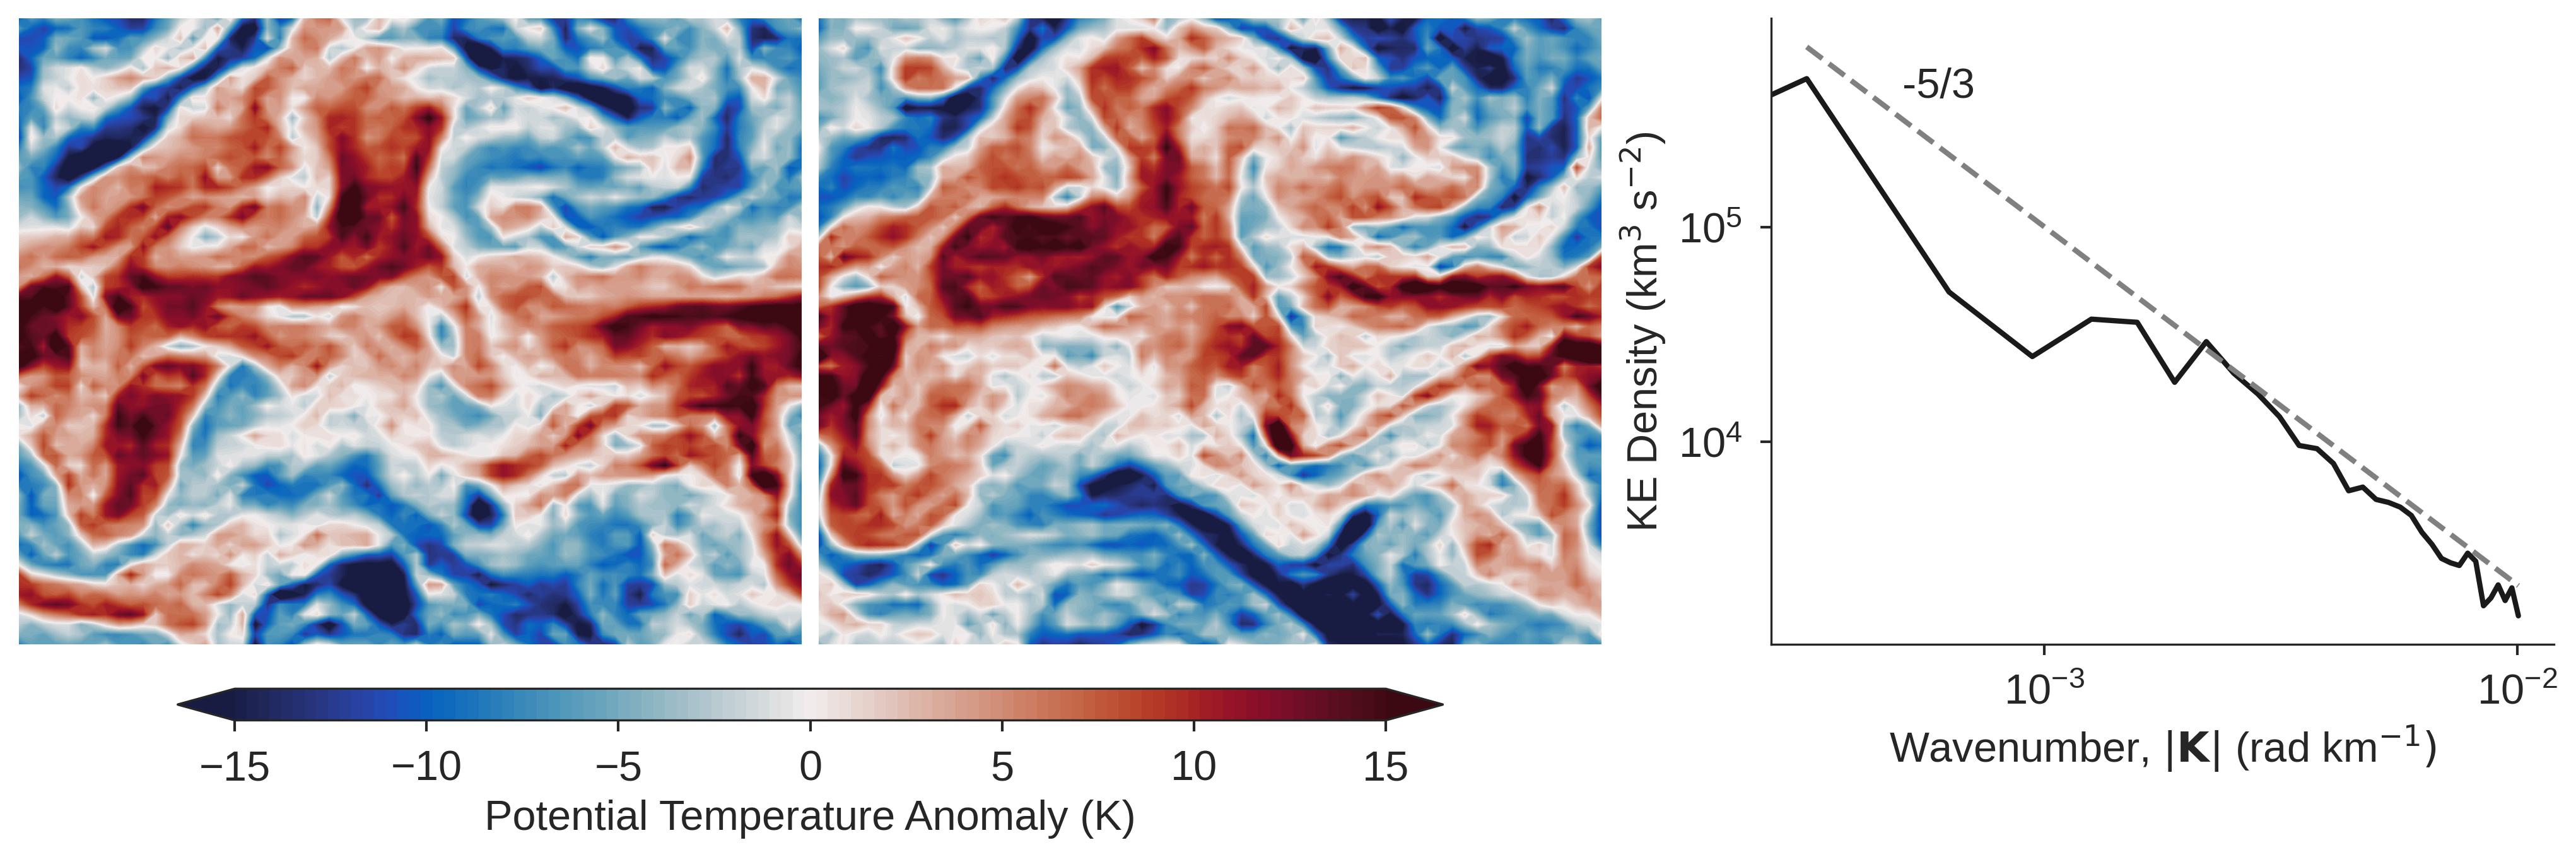
\includegraphics[width=\textwidth]{../figures/sqg_reference_plot.jpg}
    \caption{A reference snapshot from the SQG dataset. The left and middle panels
        show snapshots of potential temperature anomaly at the surface and
        top-of-troposphere layers, respectively.
        The right panel shows the kinetic energy density spectrum associated
        with this snapshot (black line), compared to
        $|\mathbf{K}|^{-5/3}$ (dashed line).
    }
    \label{fig:sqg-reference}
\end{figure}

Our model configuration is discretized in space with $N_x = N_y = 64$ and $\nvertical=2$,
uses a periodic boundary in both horizontal directions,
and uses a timestep of $\Delta t=5$~minutes.
To generate datasets for the neural networks, we initialize the model with Gaussian i.i.d.
noise and spinup for 360~days, which we define as one model year.
The spinup period is discarded, and we then generate a 25~year dataset that we partition
into training (first 15~years), validation (next 5~years), and testing
(final 5~years).
For validation and testing, we randomly select 12~hour time windows from each
respective dataset.



\section{Single Layer Recurrent and Autoregressive Neural Networks}
\label{sec:rnn-architecture}

Our goal is to develop an emulator that can reproduce the time evolution of a
dynamical system, such that its future state can be predicted from an initial
state estimate.
Therefore we use the following generic, discrete-time equations for our
recurrent and autoregressive models,
\begin{linenomath*}\begin{equation}
    \begin{aligned}
        \hidden(n+1) &= \hiddenlayer\left(
            \hidden(n), \state(n); \hyperparameters
            \right) \\
        \hat{\state}(n+1) &= \outputlayer \left( \hidden(n+1) \right) \, ,
    \end{aligned}
    \label{eq:rnn}
\end{equation}\end{linenomath*}
as in \citet{goodfellow_sequence_2016}.
Here $n\in\mathbb{Z}$ denotes a particular timestep $t = n\Delta \tau$,
where $\Delta\tau = \nsub\Delta t$ is the timestep size of the neural network,
which may be larger than $\Delta t=5$~minutes, the step size of the original model described in
\cref{sec:sqg}.
Here
$\state(n)\in\statespace$ is the state of the dynamical system and
$\hidden(n)\in\hiddenspace$ is the hidden or internal state of the network,
which is also referred to as the ``reservoir'' in RC or ``feature vector'' in
NVAR.
The generic function $\hiddenlayer(\cdot)$ evolves this hidden state forward in
time subject to the explicit
influence of the current hidden and system states, as well as the macro-scale
parameters $\hyperparameters$.
The output layer,
$\outputlayer(\cdot)$, or ``readout'' operation,
maps the hidden state back to the original state space, giving an
approximation of the target system.

During the training phase, $\state(n)$ is provided to the model at each timestep
and the misfit between the approximation and data,
$\hat{\state}(n+1) - \state(n+1)$, is used to train the weights in the output
layer.
After training, during the prediction phase, the network becomes an autonomous
system:
\begin{linenomath*}\begin{equation*}
    \hidden(n+1) = \hiddenlayer\left(
        \hidden(n), \hat{\state}(n); \hyperparameters\right) \, .
\end{equation*}\end{linenomath*}
%\todo{mention spinup ...}

The neural network architectures that we use employ common
simplifications that are relevant to the readout operator and training
procedure; we discuss these simplifications in \cref{subsec:readout}.
Additionally, we employ a similar strategy to parallelize the architecture for
high dimensional systems, and this is discussed in
\cref{subsec:parallelization}.
Finally, the specific form of $\hiddenlayer(\cdot)$ for the ESN and NVAR architectures
is provided in \cref{subsec:rc,subsec:nvar},
respectively.


\subsection{Simplified Readout and Training}
\label{subsec:readout}

The neural networks that we use employ two
simplifications relative to the generic form presented in
\cref{eq:rnn}.
First, any internal relationships encapsulated within
$\hiddenlayer(\cdot)$ are pre-defined by the macro-scale parameters,
$\hyperparameters$.
Therefore, no internal weights contained within $\hiddenlayer(\cdot)$
are learned during the formal training process.
Secondly, the readout operator is linear, such that
\begin{linenomath*}\begin{equation*}
    \outputlayer(\hidden(n)) \coloneqq \Wout \hidden(t) \, ,
\end{equation*}\end{linenomath*}
where $\Wout \in \Woutspace$ is a matrix.
The result of these two assumptions is a cost function that is quadratic with
respect to the elements of $\Wout$,
\begin{linenomath*}\begin{equation}
    \cf(\Wout) =
        \dfrac{1}{2\ntrain}\sum_{n=1}^{\ntrain}
        \norm{\Wout \hidden(n) - \state(n)}^2_2
        +
        \dfrac{\tikhonov}{2}\norm{\Wout}_\text{F}^2 \, .
    \label{eq:cost}
\end{equation}\end{linenomath*}
Here
$\norm{\mathbf{A}}_\text{F} \coloneqq
\sqrt{\text{Tr}\left(\mathbf{A}\mathbf{A}^T\right)}$
is the Frobenius norm,
$\ntrain$ is the number of time steps used for training,
$\tikhonov$ is a Tikhonov regularization parameter \citep{tikhonov_solution_1963}, chosen to improve
numerical stability and prevent overfitting.

The hidden and target states can be expressed in matrix form by concatenating
each time step ``column-wise'':
$\Hidden \coloneqq (\hidden(1) \, \hidden(2) \, \cdots \, \hidden(\ntrain))$,
and similarly\\
\noindent$\State \coloneqq (\state(1) \, \state(2) \, \cdots \, \state(\ntrain))$.
With this notation, the elements of $\Wout$ can be compactly written as the
solution to the linear ridge regression problem
\begin{linenomath*}\begin{equation}
    \Wout = \State \Hidden^T \left(\dfrac{1}{\ntrain}\Hidden\Hidden^T +
    \tikhonov\mathbf{I}\right)^{-1} \, ,
    \label{eq:ridge_regression}
\end{equation}\end{linenomath*}
although we do not form the inverse explicitly.
We instead use the \texttt{solve} function from SciPy's linear algebra module
\citep{scipy_2020}, based on testing by
\citet{platt_systematic_2022}.


\subsection{Parallelization Strategy}
\label{subsec:parallelization}

The model architectures that we use inherit the gridded structure of the target
state being emulated, and often require hidden states that are
$\mathcal{O}(10-100)$ larger.
Atmosphere and ocean GCMs typically propagate high dimensional state vectors,
$\mathcal{O}(>10^6)$,
so representing the system with a single hidden state would be intractable.
Thus, we employ a parallelization strategy to distribute the target and hidden
states across many semi-independent networks.
Our strategy follows the algorithm introduced by \citet{pathak_model-free_2018},
and follows a similar construction as \citet{arcomano_machine_2020}.
We outline the procedure here and note an illustration of the process for
the ESN architecture in \cref{fig:esn-diagram}.

We subdivide the domain into $\ngroups$ rectangular groups based on horizontal location,
akin to typical domain decomposition techniques for atmosphere and ocean
GCMs on structured grids.
Each group contains
$N_x\times N_y$ horizontal grid cells, and all $\nvertical$
vertical grid cells at each horizontal location.
The global state vector, $\state$, which consists of all state variables to be
emulated at all grid cells, is partitioned into $\ngroups$ local state vectors,
$\localstate$.
For example, \cref{fig:esn-diagram} shows a field $\state$ decomposed into nine
groups, where each group is delineated by white lines.

In order to facilitate interactions between nearby groups, each group
has a designated overlap region which consists of $\noverlap$ elements
from its neighboring groups.
The local group and overlapping points are illustrated in \cref{fig:esn-diagram}
with a black box.
The local state vectors, plus elements from the overlap region, are concatenated
to form local input state vectors, $\localinputstate$.
These local input vectors drive separate networks at each group, thereby generating
distinct hidden states for each group as follows
\begin{linenomath*}\begin{equation}
    \begin{aligned}
        \localhidden(n+1)
        &= \hiddenlayer\left(
            \localhidden(n), \localinputstate(n); \hyperparameters
        \right) \\
        \localoutput(n+1)
        &= \localWout \localhidden(n+1) \, .
    \end{aligned}
    \label{eq:local-rnn}
\end{equation}\end{linenomath*}
We make the assumption that the hyperparameters which determine internal
connections within $\hiddenlayer(\cdot)$ are globally fixed.
Therefore, the only components
that drive unique hidden states in each group are the local input vector
$\localinputstate$ and the local readout matrix, $\localWout$.

During the training phase, each group acts completely independently from one
another.
Therefore, the training process is embarrassingly parallel and allows us to
scale the problem to arbitrarily large state vectors across a distributed
computing system, subject to resource constraints.
During the prediction phase, neighboring elements must be passed between
groups in order to fill each overlap region at each time step.
%We note that this requirement is not overbearing, as GCMs require similar
%message passing between neighboring processes in order to compute spatial
%derivatives and perform interpolation.

\subsection{Nonlinear Vector Autoregression Design}
\label{subsec:nvar}

%In \citet{gauthier_next_2021} this RNN is referred to as ``Next Generation
%Reservoir Computing'' because it is motivated by the RC framework.
%However, we note (as do the authors), that this is identical to the already
%existing Nonlinear Vector Autoregression (NVAR), and so we refer to this general architecture as
%such.
As in \citet{gauthier_next_2021,chen_next_2022}, we form the hidden state using
polynomial combinations of the time-lagged input state.
We explain this process with a simple example using a two variable system,
$\inputstate(n) = [u_0(n), u_1(n)]^T$,
a maximum polynomial degree,
$\maxpolynomial=2$, and a generic maximum number of lagged states, $\maxlag$:
\begin{linenomath*}\begin{equation}
    \begin{aligned}
        \localhidden(n+1)
        =
        [&1, \\
        % linear
         &u_0(n), \,\, u_1(n), \,\,
        u_0(n-1),\,\, u_1(n-1), \,\,
        \cdots \,\,
        u_0(n-\maxlag), \,\, u_1(n-\maxlag), \\
        % quadratic
         &u_0^2(n), \,\, u_1^2(n), \,\, u_0(n)u_1(n), \,\,
        u_0^2(n-1), \,\, \cdots \,\, u_1^2(n-\nlag) \\
         &u_0(n)u_0(n-1), \,\,
        u_0(n)u_1(n-1), \,\, \cdots \,\, u_0(n-\nlag)u_1(n), \,\,\cdots
        ] \\
        \localoutput(n+1) = &\localWout \localhidden(n+1) \, .
    \end{aligned}
\end{equation}\end{linenomath*}
Clearly, the size of the hidden state vector grows rapidly with
$\maxpolynomial$ and $\nlag$,
even for relatively low dimensional systems
\citep<see supplemental material of>[for explicit calculations]{chen_next_2022}.
We therefore make a simplification to the generic polynomial NVAR model.
That is, we only represent nonlinear interactions between points that lie
within a given radius between one another, defined by the number of neighboring
points, $\nneighbor$.
As a simple example, with $\nneighbor=1$ and $\maxlag=0$, the quadratic elements of a periodic, four variable
system would be
\begin{linenomath*}\begin{equation*}
    u_0^2, \,\, u_1^2, \,\, u_2^2, \,\, u_3^2, \,\,
    u_0u_1, \,\, u_0u_3, \,\, u_1u_2, \,\, u_2u_3
\end{equation*}\end{linenomath*}
ignoring ``non-local'' interactions such as $u_0u_2$.
In order to make this parameter consistent with the overlap region in the
parallelization scheme (\cref{subsec:parallelization}),
we set $\nneighbor = \noverlap = 1$ \red{SEE TABLE}.

All of the remaining macro-scale parameters that determine the NVAR performance are
\begin{linenomath*}\begin{equation*}
    \nvarparams =
    \{ \maxpolynomial, \maxlag, \tikhonov \} \, .
\end{equation*}\end{linenomath*}
By using the preconditioning scheme introduced in \citet{chen_next_2022},
we found results to be insensitive to the Tikhonov parameter $\tikhonov$, and so
we fix this to $\tikhonov = 10^{-4}$.
As noted earlier, we set $\maxpolynomial = 2$.
Our assumption behind this decision is that the NVAR model will be able to learn local
quantities like gradients and fluxes between neighboring grid cells.
Based on the results from \citet{chen_next_2022},
the NVAR model should then be able to use this information to construct
arbitrarily complex time stepping schemes as a function of $\nlag$.
Because of its explicit nature, we manually vary this
integer parameter to understand how memory impacts NVAR prediction skill.


\subsection{Echo State Network Design}
\label{subsec:rc}


\begin{figure}
    \centering
    \begin{overpic}[width=.8\textwidth]{../figures/esn-diagram.pdf}

        \put(25, 40) {\footnotesize $\localinputstate(n)$}
        \put(32.5, 31) {\footnotesize $\inputmatrix$}

        \put(34, 18) {\footnotesize $\adjacency$}
        \put(18.5, 11) {\footnotesize$\localhidden(n)$}

        \put(47, 17) {\footnotesize $\tanh(\cdot)$}
        \put(54.5, 22) {\footnotesize$\alpha$}
        \put(56, 6) {\footnotesize $1-\alpha$}

        \put(55, 32) {\footnotesize $\localhidden(n+1)$}
        \put(62.75, 20) {\footnotesize $\localWout$}
        \put(65, 29) {\footnotesize $\localoutput(n+1)$}
    \end{overpic}
    \caption{An illustration of the ESN architecture used, as it
        is applied to each local group throughout the domain.
        The domain is decomposed purely based on horizontal location, so the
        illustration shows a single horizontal slice, but note that each group
        contains all $\nvertical$ vertical levels.
        In this example, there are nine groups delineated by the white lines on
        the 2D slice on the left.
        The black box denotes the group being operated on, which includes a
        region of width $\noverlap$ that overlaps with neighboring groups.
        At timestep $n$, the group is flattened to make the input vector
        $\localinputstate(n)$, which is
        mapped into the ESN via $\inputmatrix$.
        The output $\localoutput(n+1)$ is expanded to fill its position in the global
        domain.
    }
    \label{fig:esn-diagram}
\end{figure}

Our ESN architecture is illustrated in \cref{fig:esn-diagram}, and is defined as
follows
\begin{linenomath*}\begin{equation}
    \begin{aligned}
        \localhidden(n+1)
        &=
        \left(1-\leak\right)\localhidden(n)
        +
        \leak \tanh\left(
            \adjacency \localhidden(n) + \inputmatrix \localinputstate(n) + \biasvector
            \right)
             \\
        \localoutput(n+1)
        &= \localWout \localhidden(n+1) \, .
    \end{aligned}
    \label{eq:rc}
\end{equation}\end{linenomath*}
Here
$\leak\in[0,1]$ is a leak parameter,
$\adjacency \in \mathbb{R}^{\nhidden\times\nhidden}$ is an adjacency matrix that
determines the internal connections between the nodes of the hidden state,
$\inputmatrix \in \mathbb{R}^{\nhidden\times\ninputstate}$ maps the input vector
into the higher dimensional hidden state,
and $\biasvector\in\mathbb{R}^{\nhidden}$
is the bias vector with elements
$\biasvectorelement_i \sim \mathcal{U}(-\bias,\bias)$.
Finally, we note that ESNs require a spinup period before generating
predictions, so we specify a 10~day spinup period for all validation and testing
samples.
%Given the parallelization scheme described in \cref{subsec:parallelization},
%the network can be considered as $\ngroups$ interacting ESNs, each with
%$\nhidden$ nodes, or as one network with $\ngroups\times\nhidden$ nodes.

Two scalar parameters, $\spectralradius$ and $\inputscaling$,
are used to control the scaling of the adjacency and input matrices,
respectively.
These parameters have dramatic influence on the ESNs prediction skill, since their
values influence the network's memory and stability
\citep{lukosevicius_practical_2012,hermans_memory_2010}.
Here we first normalize the matrices by their largest singular value, and then
apply the scaling parameters as follows
\begin{linenomath*}\begin{equation*}
    \adjacency \coloneqq
    \dfrac{\spectralradius}{\sigma_{max}\left(\hat{\adjacency}\right)}
    \hat{\adjacency}
    \qquad
    \inputmatrix \coloneqq
    \dfrac{\sigma}{\sigma_{max}\left(\hat{\mathbf{W}}_\text{in}\right)}
    \hat{\mathbf{W}}_\text{in} \,
\end{equation*}\end{linenomath*}
where the elements of $\hat{\mathbf{W}}_\text{in}$
are initialized with elements $\hat{w}_{i,j}\sim\mathcal{U}(-1,1)$.
The initial adjacency matrix is generated similarly, except that the indices
$i,j$ are randomly chosen such that $\hat{\adjacency}$ attains a specified
sparsity.
Here we set the matrix sparsity to $1 - \kappa / \nhidden$, with $\kappa=6$,
following the success of very sparsely connected adjacency matrices as shown by
\citet{griffith_forecasting_2019}.
By first normalizing the matrices by the largest singular value, the parameters
$\spectralradius$ and $\inputscaling$ re-scale the induced 2-norm of
the matrix.
This normalization is not standard in the ESN literature, but we found that it
helped improve prediction skill.
We provide further discussion of this process in \cref{sec:new_methods}.

In summary, the macro-scale parameters that determine the overall
characteristics of the ESN are

\begin{linenomath*}\begin{equation}
    \esnparams =
    \{ \spectralradius, \inputscaling, \bias, \leak, \tikhonov \} \,
    ,
    \label{eq:rc-hyperparameters}
\end{equation}\end{linenomath*}
which are globally fixed for all groups.
Due to the high sensitivity of ESN prediction skill to these parameter values,
we follow the general optimization framework described by
\citet{platt_systematic_2022} to determine approximately optimal values.
We use the Bayesian optimization algorithm outlined by
\citet{jones_efficient_1998} and implemented by \citet{bouhlel_python_2019} to tune them.
This process is discussed in \cref{sec:esn-results}, \red{and more details are
provided in the supplement}.

\section{Nonlinear Vector Autoregression Prediction Skill}
\label{sec:nvar-results}

In this section we show the prediction skill of the polynomial based NVAR architecture
described in \cref{subsec:nvar}.
To quantitatively evaluate each forecast, we compute
the normalized root-mean-square error (NRMSE)
\begin{linenomath*}\begin{equation}
    \text{NRMSE}(n) = \sqrt{\dfrac{1}{\nstate}\sum_{i=1}^{\nstate}\left(
        \dfrac{\hat{v}_i(n) - v_i(n)}{SD}
        \right)^2 } \, ,
    \label{eq:nrmse}
\end{equation}\end{linenomath*}
which is averaged over each spatial dimension, succinctly represented as a
summation over $\nstate$, and normalized by the standard deviation, $SD$,
computed from the true trajectory over time and all spatial dimensions.
Additionally, we compute the relative error in terms of the kinetic energy
(KE) density spectrum,
\begin{linenomath*}\begin{equation}
    \text{KE Relative Error}(k, n) =
    \dfrac{\hat{E}(n, k) - E(n, k)}{|E(n,k)|} \, ,
    \label{eq:ke_relerr}
\end{equation}\end{linenomath*}
where $E(n,k)$ and $\hat{E}(n,k)$ are the true and predicted KE density coefficients
for each timestep $n$ and wavenumber $k$, respectively (e.g., as in the right
panel of \cref{fig:sqg-reference}).
Note that $|\cdot|$ denotes the absolute value operation,
and we retain the sign of the error in order to show a sense of the
spectral error in each prediction.

We compute these quantities based on 50, 12~hour predictions, initialized from a random
set of initial conditions taken from an unseen test dataset.
To compactly visualize the skill over all samples, each lineplot in the
following subsections shows a sample-average value with a solid line, and the
99\% confidence interval with shading.

\subsection{Temporal Subsampling}
\label{subsec:nvar-subsampling}


\begin{figure}
    \centering
    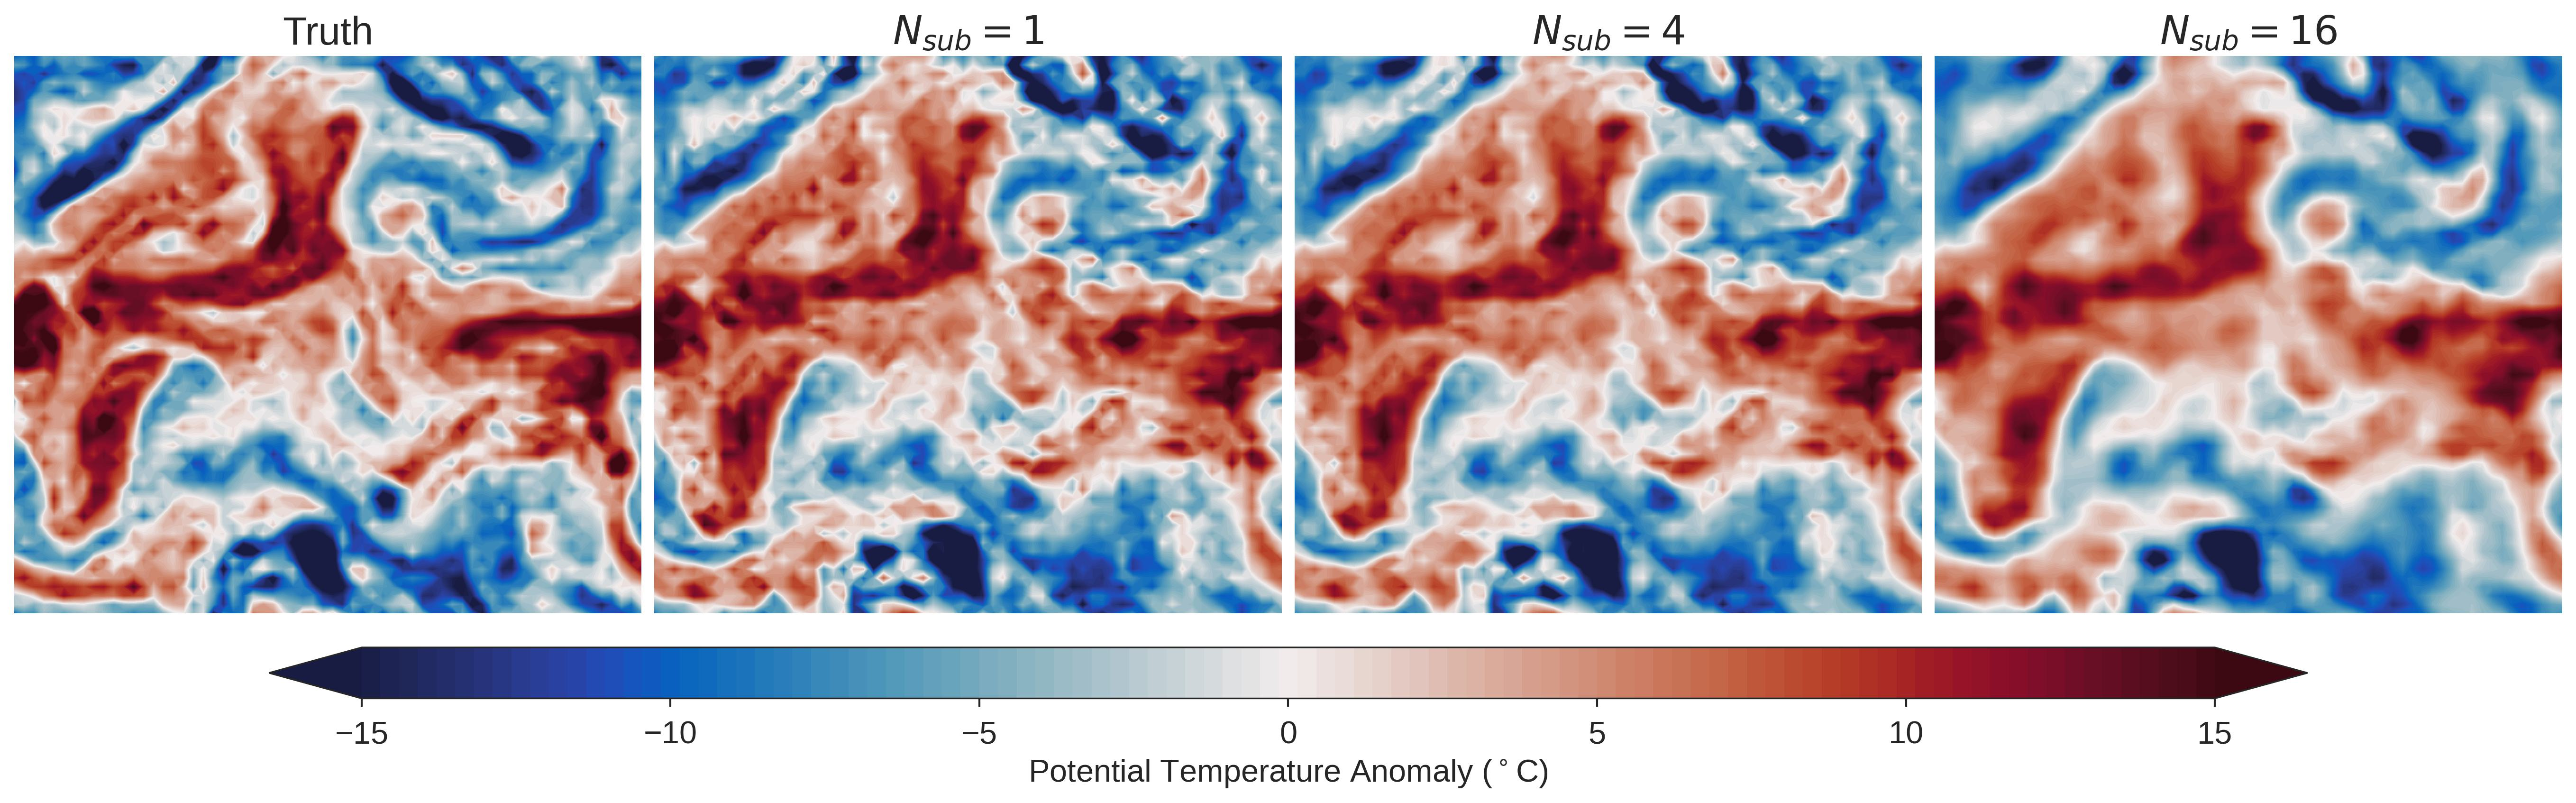
\includegraphics[width=\textwidth]{../figures/nvar_4hr_snap.jpg}
    \caption{One sample NVAR prediction from the test dataset for $\nsub =
        1,4,16$, shown in the second, third, and fourth rows at a lead time of 4~hours.
        The corresponding truth is shown in the far left panel.
        Here $\maxlag=1$ and only the surface level is shown.
    }
    \label{fig:nvar_qualitative}
\end{figure}

\begin{figure}
    \centering
    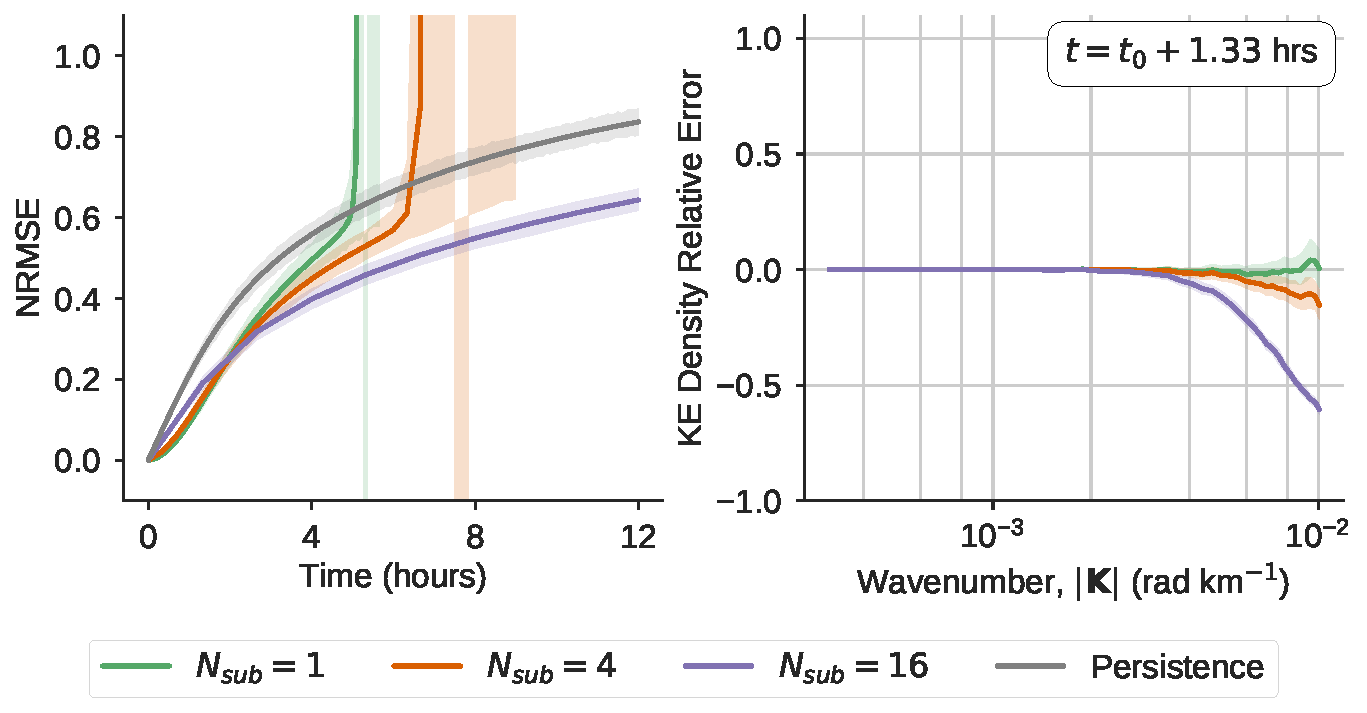
\includegraphics[width=.8\textwidth]{../figures/nvar-nrmse-and-kere.pdf}
    \caption{NRMSE (\cref{eq:nrmse}; left) and KE density
        relative error (\cref{eq:ke_relerr}; right)
        indicating prediction skill of the NVAR
        architecture using 50~samples from the test dataset.
        Solid lines indicate averages and shading indicates 99\% confidence
        interval.
        Here $\nlag=1$.
    }
    \label{fig:nvar_nrmse}
\end{figure}

% Describe the big plot
\cref{fig:nvar_qualitative} shows a qualitative comparison of NVAR predictions
as a function of $\nsub$, i.e., how frequently the training data are sampled and
the model makes predictions.
For this figure, we set $\nlag=1$, and note that both the NRMSE and a snapshot
of the KE density relative error corresponding to this configuration are shown in
\cref{fig:nvar_nrmse}.

At the model timestep ($\Delta \tau = \Delta t = 5$~min; $\nsub=1$), the NVAR predictions are
qualitatively similar to the truth for short forecast lead times.
That is, the NRMSE is near 0, and
many of the small scale features that exist in the truth are also evident
in the predictions.
However, at longer lead times the predictions become unstable.
NRMSE spikes rapidly at about 4~hours after numerical instabilities are
generated, which causes the NVAR model to produce physically unrealistic results.
For reference, \cref{fig:nvar_instabilities} shows a view of what these
numerical instabilities look like at their onset.
\todo{Do you think this figure is necessary?}

\begin{figure}
    \centering
    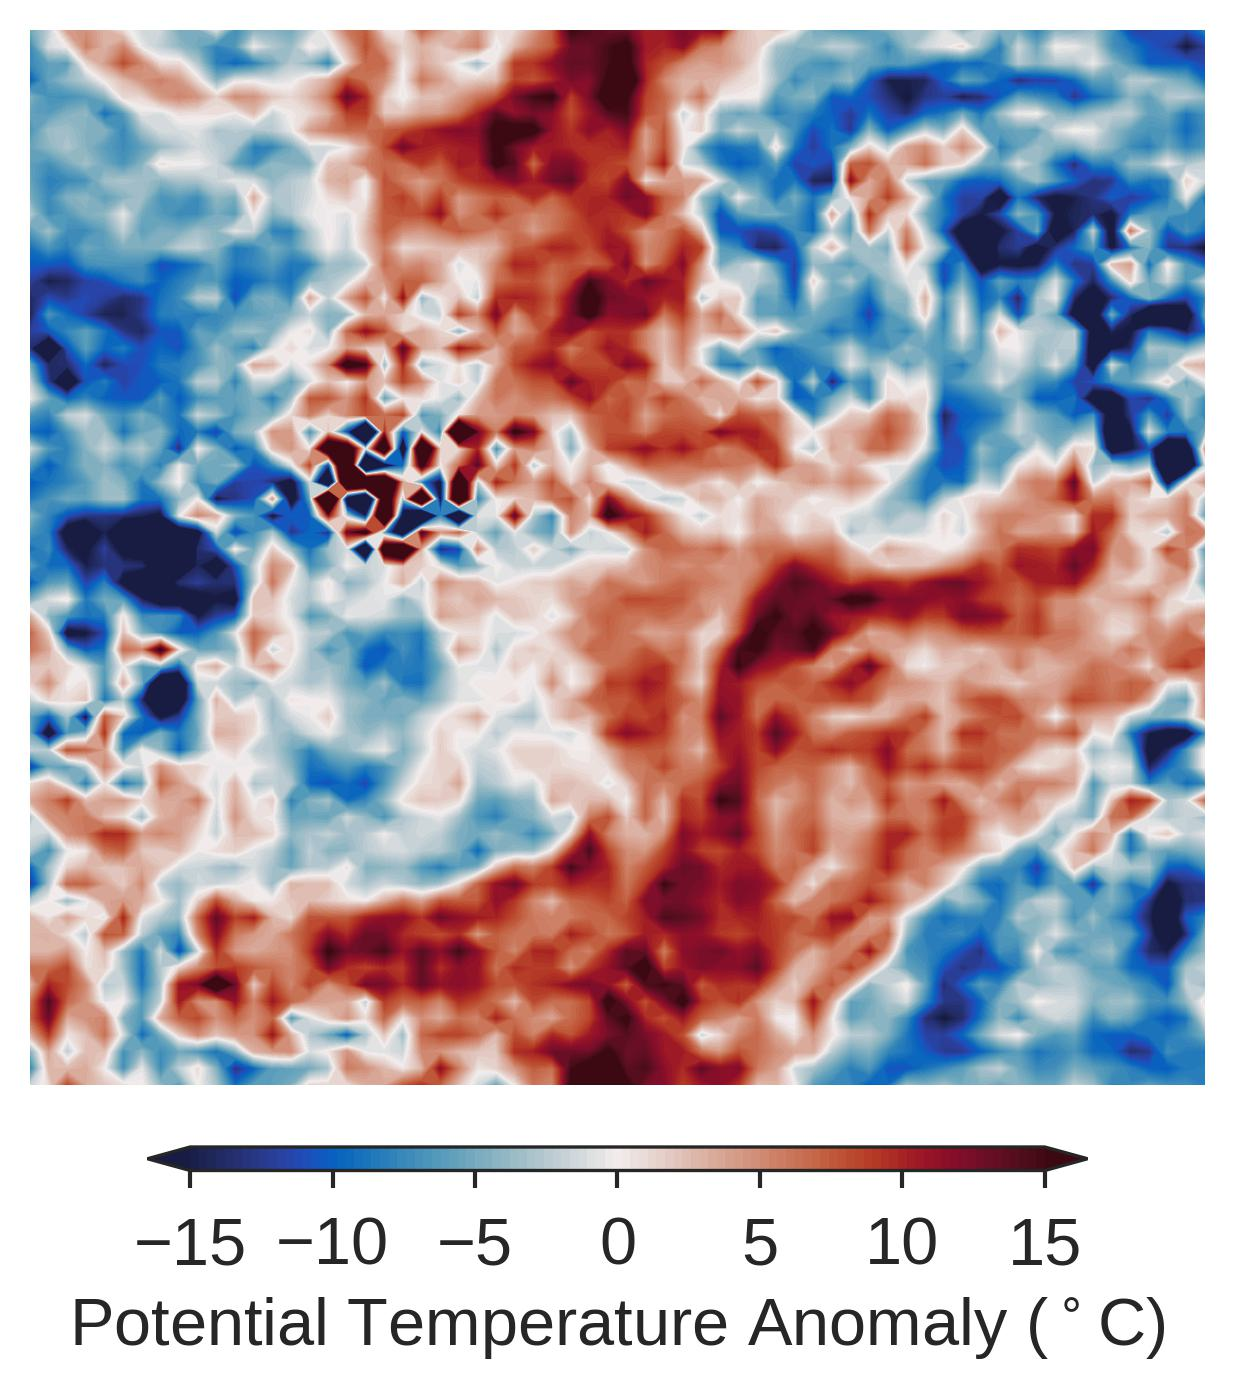
\includegraphics[width=.3\textwidth]{../figures/nvar_instabilities.jpg}
    \caption{A view of the numerical instabilities generated by the NVAR model.
        This particular example occurs after 8~hours, given the same initial
        conditions in \cref{fig:nvar_qualitative} and $\nsub=1; \nlag=1$.
    }

    \label{fig:nvar_instabilities}
\end{figure}

As the temporal resolution of the data is reduced, i.e., as $\nsub$ increases,
the predictions are generally stable for a longer period of time.
\cref{fig:nvar_nrmse} shows that for $\nsub=4$, predictions are stable for roughly
6~hours, and for $\nsub=16$ no predictions generate numerical instabilities over the
12~hour window.
However, this stability comes with a cost: as the temporal resolution is
reduced, the model's representation of small scale features diminishes as these
features become more blurry or smooth.
This blurring effect is apparent in \cref{fig:nvar_qualitative}, where the
prediction is qualitatively more blurry as
$\nsub$ increases in each panel from left to right.

This smoothing behavior is captured quantitatively in the right panel of
\cref{fig:nvar_nrmse},
which shows the KE relative error as in \cref{eq:ke_nrmse}.
Here, we show the KE relative error after only 1.33~hours to show the behavior
before instabilities dominate the $\nsub=1$ predictions.
The plot indicates the degree of spectral bias in each solution, which is
largest at the smaller spatial scales, corresponding to higher wave numbers.

At $\nsub=1$ there is a small positive bias at the smallest resolved spatial
scales, indicating that this is when numerical instabilities are starting to
generate.
The subsampled runs, $\nsub=\{4,16\}$, show a negative bias, which corresponds
to a damped energy spectrum at the scales that are not resolved in the
qualitatively smooth predictions shown in \cref{fig:nvar_qualitative}.
This negative bias is clearly larger with higher subsampling, or reduced
temporal resolution.


\subsection{Prediction Skill as a Function of Memory}
\label{subsec:nvar-memory}

A key feature of RNNs and autoregressive models is that they retain memory of
previous system states.
Given the explicit nature of the NVAR architecture, we explore the effect of
adding memory by increasing $\nlag$, the number of lagged states used to create the
feature vector.
We first summarize how memory impacts prediction skill in
\cref{fig:nvar_nrmse_vs_lag}, which shows the NRMSE as a
function of $\nlag$ (colors) for each
subsampling factor $\nsub = \{1, 4, 16\}$ (panels).
For any value of $\nsub$, adding memory (increasing $\nlag$) reduces
the short term error.
However, adding memory also tends to increase error by the end of the forecast,
often leading to the development of numerical instabilities and an
incoherent solution.
Similarly, for any fixed value of $\nlag$, increasing the temporal resolution
(decreasing $\nsub$) shows the same behavior.

\begin{figure}
    \centering
    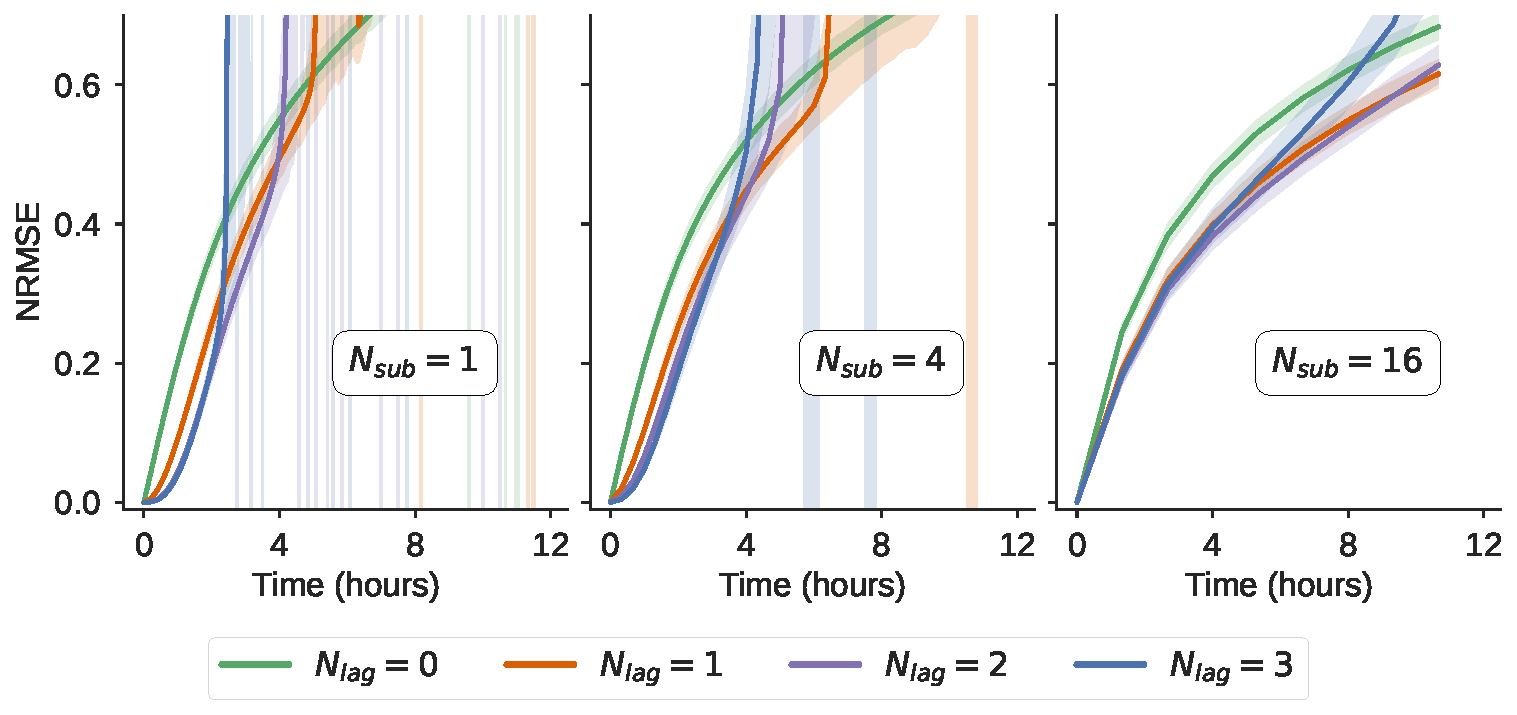
\includegraphics[width=\textwidth]{../figures/nvar_nrmse_vs_memory.pdf}
    \caption{NRMSE computed using NVAR at various temporal resolutions
        ($\nsub$; columns) and with variable memory capacities ($\nlag$;
        colors).
    }
    \label{fig:nvar_nrmse_vs_lag}
\end{figure}

To shed some light on how this additional memory impacts the solution,
we show the KE relative error
for the case of $\nsub=16$ as a function of time (panels) and $\nlag$ (colors)
in \cref{fig:nvar_ke_vs_lag}.
For about the first 4~hours, increasing memory improves prediction skill at all
spatial scales.
However, beyond this point, the overall NRMSE grows rapidly, the improvement
at small scales ($|\mathbf{K}|>4\cdot10^{-3}$~rad~km$^{-1}$) is more muted,
and error is propagated rapidly into the larger spatial scales.

We surmise that adding memory degrades the long term prediction skill because
the relationship between points further back in history are governed by higher
order nonlinear interactions that are incorrectly represented by
the simple local-quadratic relation that is used here.
As more terms are added that are incorrectly represented, the model becomes
more and more unstable.
The question is therefore how to retain the short term benefit of added memory
capacity throughout the forecast horizon while maintaining a stable trajectory.
While it may seem natural to explore higher order polynomials to
properly represent this history, we do not explore this further because the size
of the feature vector grows dramatically with the polynomial order
\citep{chen_next_2022}.
Another option would be to explore entirely different basis functions.
While this could be a potential option for future work, we note the findings of
\citet{zhang_catch-22_2022}, who show the extreme sensitivity of NVAR to the
form of nonlinearity imposed.
Given that it is an entirely open question on how to represent the smallest
scales of geophysical turbulence, we do not explore other basis functions, and
instead turn to the more general ESN architecture.

\begin{figure}
    \centering
    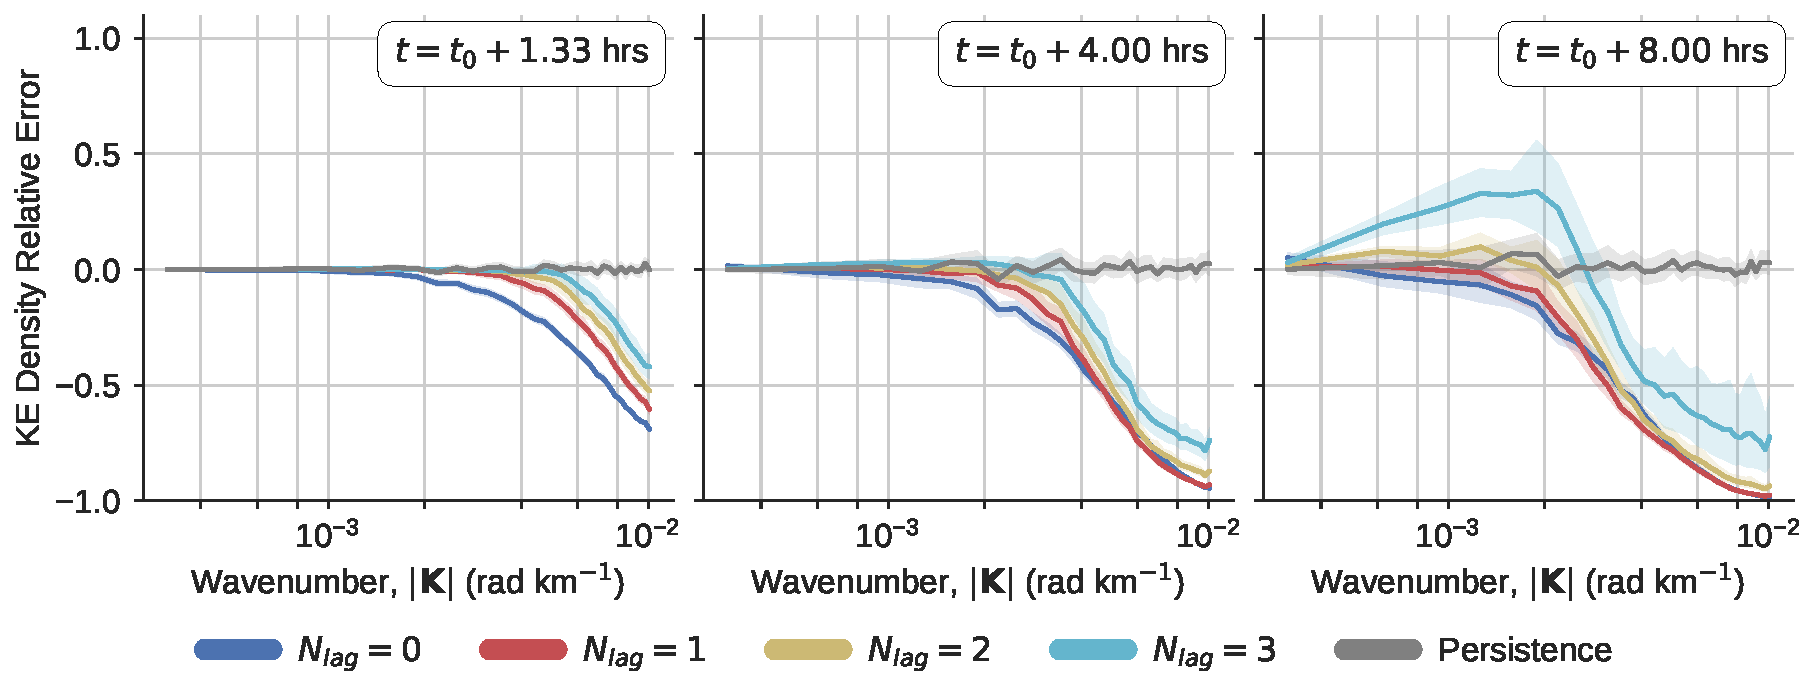
\includegraphics[width=\textwidth]{../figures/nvar_ke_relerr_vs_lag.pdf}
    \caption{Kinetic energy density relative error with $\nsub=16$ at various
        timesteps (columns) and memory capacity ($\nlag$; colors).
    }
    \label{fig:nvar_ke_vs_lag}
\end{figure}

\section{ESN Results}
\label{sec:esn-results}

In this section we show the prediction skill of the more generic ESN
architecture outlined in \cref{subsec:rc}.
Here we use similar metrics as in \cref{sec:nvar-results} to evaluate the ESN
skill, except that we show time averaged quantitative metrics because all of the
ESN predictions are stable for the full 12~hour forecast horizon.
That is, when shown as a single distriubtion rather than a time series, NRMSE is reported as
\begin{linenomath*}\begin{equation}
    \text{NRMSE} = \sqrt{
            \dfrac{1}{\ntime\nstate}\sum_{n=1}^{\ntime}\sum_{i=1}^{\nstate}\left(
        \dfrac{\hat{v}_i(n) - v_i(n)}{SD}
        \right)^2 } \, ,
    \label{eq:total-nrmse} \, ,
\end{equation}\end{linenomath*}
where $\ntime$ consists of the number of timesteps in the trajectory, whether
from the validation or test dataset.
In order to characterize spectral error, we show the KE relative error as in
\cref{sec:nvar-results}.
Additionally, we show the NRMSE in terms of the KE density spectrum as follows
\begin{linenomath*}\begin{equation}
    \text{KE\_NRMSE} = \sqrt{
            \dfrac{1}{\ntime\nk}\sum_{n=1}^{\ntime}\sum_{k=1}^{\nk}\left(
            \dfrac{\hat{E}(n, k) - E(n, k)}{SD(k)}
            \right)^2} \, ,
    \label{eq:ke_nrmse}
\end{equation}\end{linenomath*}
where $\nk$ is the number of spectral coefficients and $SD(k)$ is the temporal
standard deviation of each spectral coefficient throughout the test trajectory.
As in \cref{sec:nvar-results}, all distributions and lineplots indicate
prediction skill from 50 randomly selected initial conditions from an unseen
test dataset.


\subsection{Soft Constraints on Spectral Error}
\label{subsec:esn-ego}

% Here we present ESN results, using mainly the two metrics used to evaluate
% NVAR
It is well known that ESN prediction skill is highly dependent on the global or
``macro-scale'' parameters noted in
\cref{eq:rc-hyperparameters},
\citep<$\esnparams$, e.g.>[]{platt_systematic_2022,lukosevicius_practical_2012}.
Following the success of previous studies in using Bayesian optimization methods
to systematically tune these parameters
\citep{platt_systematic_2022,penny_integrating_2022,griffith_forecasting_2019},
we use the algorithm outlined by \citet{jones_efficient_1998} and implemented by
\citet{bouhlel_python_2019} to find optimal parameter values.

More recently \red{PLATT} showed that constraining these macro-scale
parameters using global invariant properties of the underlying system leads the
optimization algorithm to select parameters that generalize well to unseen test
data.
In their work, the authors were successful in using the largest positive
Lyapunov exponent, and to a lesser extent the fractal dimension of the system.
Because of the focus on resolved scales in this work, we take a similar
approach, but test the effect of constraining the ESN to the KE density
spectral coefficients.
Specifically, we implement the following two stage training process.
At each step, the macro-scale parameters, $\esnparams$, are fixed, and the
``micro-scale'' parameters $\Wout$ are obtained by minimizing \cref{eq:cost}.
This readout matrix is then used to make forecasts from randomly selected
initial conditions from a validation dataset.
The skill of each of these forecasts is captured by the macro-scale cost
function
\begin{linenomath*}\begin{equation}
    \cf_\text{macro}(\esnparams) = \dfrac{1}{\nmacro}
    \sum_{j=1}^{\nmacro}
    \left\{
        \text{NRMSE}(j) + \gamma \text{KE\_NRMSE}(j)
    \right\}
    \label{eq:macro-cost} \, ,
\end{equation}\end{linenomath*}
where NRMSE and KE\_NRMSE are defined in \cref{eq:total-nrmse,eq:ke_nrmse},
$\nmacro$ is the number of forecasts used in the validation set, and $\gamma$ is
a hyperparameter that determintes how much to penalize deviations
from the true KE density spectrum.
The value of $\macrocost$ is then used within the Bayesian optimization
algorithm, which reiterates the whole optimization process with new values for
$\esnparams$ until an optimal value is found or the maximum number of
iterations is reached.
See \red{THE APPENDIX} for more details on our optimization configuration, and
note that we go through this optimization procudure for each unique ESN configuration
throughout \cref{sec:esn-results} (i.e., for each $\nsub$ and each $\gamma$
value).

\cref{fig:rc_qualitative_nsub01} shows a qualitative view of how penalizing the
KE density impacts ESN prediction skill when it operates at the original
timestep of the SQG model (i.e., $\nsub=1$).
At $\gamma=0$, only the ESN parameters are selected based on NRMSE alone, and
the prediction is somewhat blurry.
However, as $\gamma$ increases to $10^{-1}$, the prediction becomes sharper as
the small scale features are seemingly better resolved.

\cref{fig:rc_quantiative_nsub01} gives a quantitative view of how the KE density
penalty changes ESN prediction skill, once again with $\nsub=1$.
The first two panels show that there is a clear tradeoff between NRMSE and KE error:
as $\gamma$ increases the NRMSE decreases but the spectral representation improves.
The final panel in \cref{fig:rc_quantiative_nsub01}
shows that the spatial scales at which the spectral error manifests in these
different solutions.
When $\gamma=0$, the ESN global parameters are chosen to minimize NRMSE, leading
to blurry predictions and a dampened spectrum at the higher wavenumbers,
especially for $|\mathbf{K}| > 2\cdot10^{-3}$~rad~km$^{-1}$.
On the other hand, when $\gamma = 10^{-1}$, the global parameters are chosen to
minimize both NRMSE and KE density error.
In this case, KE relative error is reduced by more than a factor of two and the
spectral bias at higher wavenumbers is much more muted.
However, the tradeoff for this reduced spectral error is larger NRMSE, resulting
from slight mismatches in the position of features in the forecast.
We note that using larger values of $\gamma$ produces similar results to
$\gamma=10^{-1}$.

%However, as time progresses through the 12~hour forecast window,
%the KE relative error increases slightly at the larger spatial scales,
%$|\mathbf{K}| \lessapprox 10^{-3}$~rad~km$^{-1}$ (not shown),
%and this error is what causes NRMSE to be roughly 10\% higher in the case where
%$\gamma=10^{-1}$ than $\gamma=0$.

\begin{figure}
    \centering
    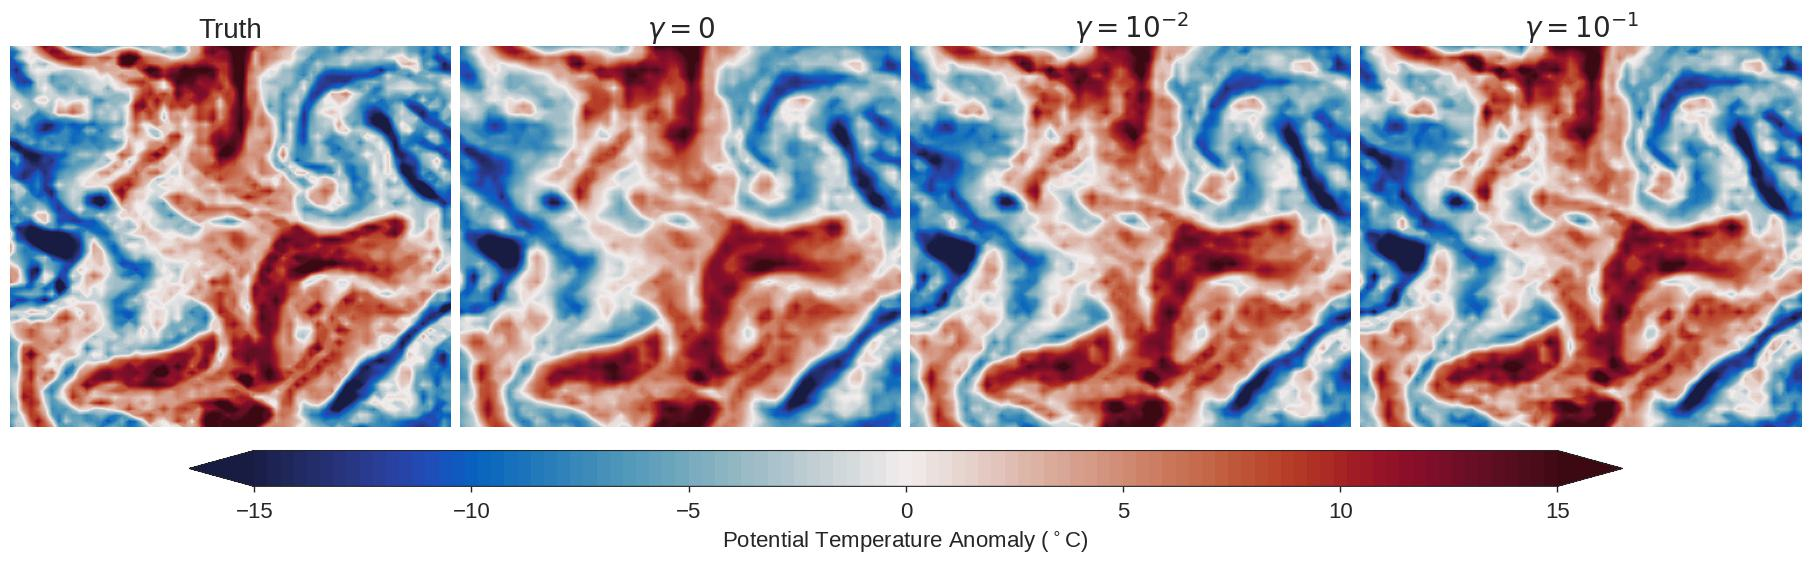
\includegraphics[width=\textwidth]{../figures/rc_qualitative_gamma.jpg}
    \caption{
        One sample prediction from the test dataset, where each panel shows
        potential temperature in the truth (left) and subsequently for
        ESN predictions with parameters optimized using
        $\gamma=\{0, 10^{-2}, 10^{-1}\}$ in \cref{eq:macro-cost}.
        Each panel shows the prediction at a forecast lead time of 4~hours,
        using the same initial conditions as in \cref{fig:nvar_qualitative}.
        Here, the ESN is evaluated at the SQG model timestep, i.e., $\nsub=1$.
    }
    \label{fig:rc_qualitative_nsub01}
\end{figure}

\begin{figure}
    \centering
    \begin{overpic}[width=\textwidth]{../figures/rc_all_nsub01.pdf}
        \put( 6, 27) {(a)}
        \put(40, 27) {(b)}
        \put(72, 27) {(c)}
    \end{overpic}
    \caption{
        Quantitative comparison of ESN predictions at $\nsub=1$ with macro-scale
        parameters
        chosen using different values of $\gamma$ in \cref{eq:macro-cost}.
        NRMSE (\cref{eq:total-nrmse}; a), KE\_NRMSE (\cref{eq:ke_nrmse}; b), and
        KE relative error (\cref{eq:ke_relerr}; c) highlight the tradeoff
        between minimizing NRMSE and spectral bias.
        Note that the KE relative error in (c) is shown at 4~hours to provide
        direct comparison to the snapshots in \cref{fig:rc_qualitative_nsub01}.
    }
    \label{fig:rc_quantiative_nsub01}
\end{figure}



\subsection{The effect of temporal subsampling}
\label{subsec:esn-subsampling}


The NVAR predictions shown in \cref{subsec:nvar-subsampling} indicated that
subsampling the training data increases spectral bias.
However, the architecture was not specifically designed or constrained to
have a good spectral representation of the underlying dynamics.
On the other hand, the previous section (\cref{subsec:esn-ego})
showed that spectral bias can be reduced by optimizing the global ESN parameters
to the true KE density spectrum.
Given these two results, we explore the following question: does temporal subsampling still
increase spectral bias in the more general ESN framework, even when parameters
are chosen to minimize this bias?

\cref{fig:rc_qualitative_gamma0.1} and \cref{fig:rc_quantiative_gamma0.1}
show that even when the macro-scale parameters are chosen to prioritize the KE
density representation (i.e., $\gamma = 0.1$ is fixed),
temporal subsampling does lead to an apparently inescapable spectral bias.
This effect is shown qualitatively in \cref{fig:rc_qualitative_gamma0.1},
where the predictions become
smoother as the temporal subsampling factor, $\nsub$, increases.
The effect is similar to what was seen with NVAR except the blurring effect is
less intense.
Quantitatively, \cref{fig:rc_quantiative_gamma0.1}(b) shows that as $\nsub$
increases, error in KE density spectrum generally increases, while panel (c) shows that this KE
error is concentrated in the small spatial scales,
$|\mathbf{K}| > 2\cdot10^{-3}$~rad~km$^{-1}$.
We note that the degree of spectral bias at $\nsub=16$ is smaller than what was
achieved with NVAR for the same $\nsub$ value, cf. \cref{fig:nvar_ke_vs_lag},
indicating that the optimization was successful in reducing the spectral bias.

\begin{figure}
    \centering
    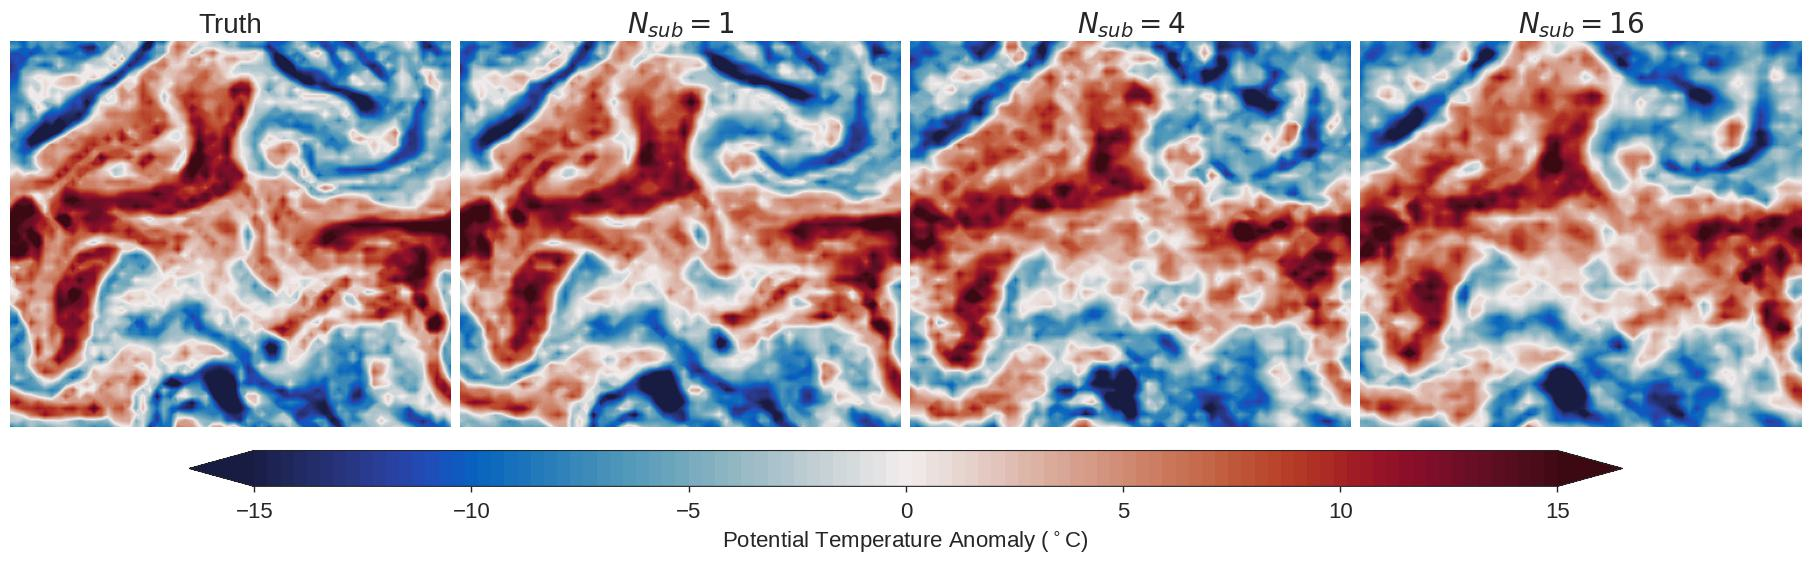
\includegraphics[width=\textwidth]{../figures/rc_qualitative_nsub.jpg}
    \caption{One sample prediction from the test dataset, exactly as in
        \cref{fig:rc_qualitative_nsub01}, except here $\gamma=10^{-1}$ is fixed, and
        the temporal subsampling factor is varied: $\nsub=\{1,4,16\}$.
    }
    \label{fig:rc_qualitative_gamma0.1}
\end{figure}

\begin{figure}
    \centering
    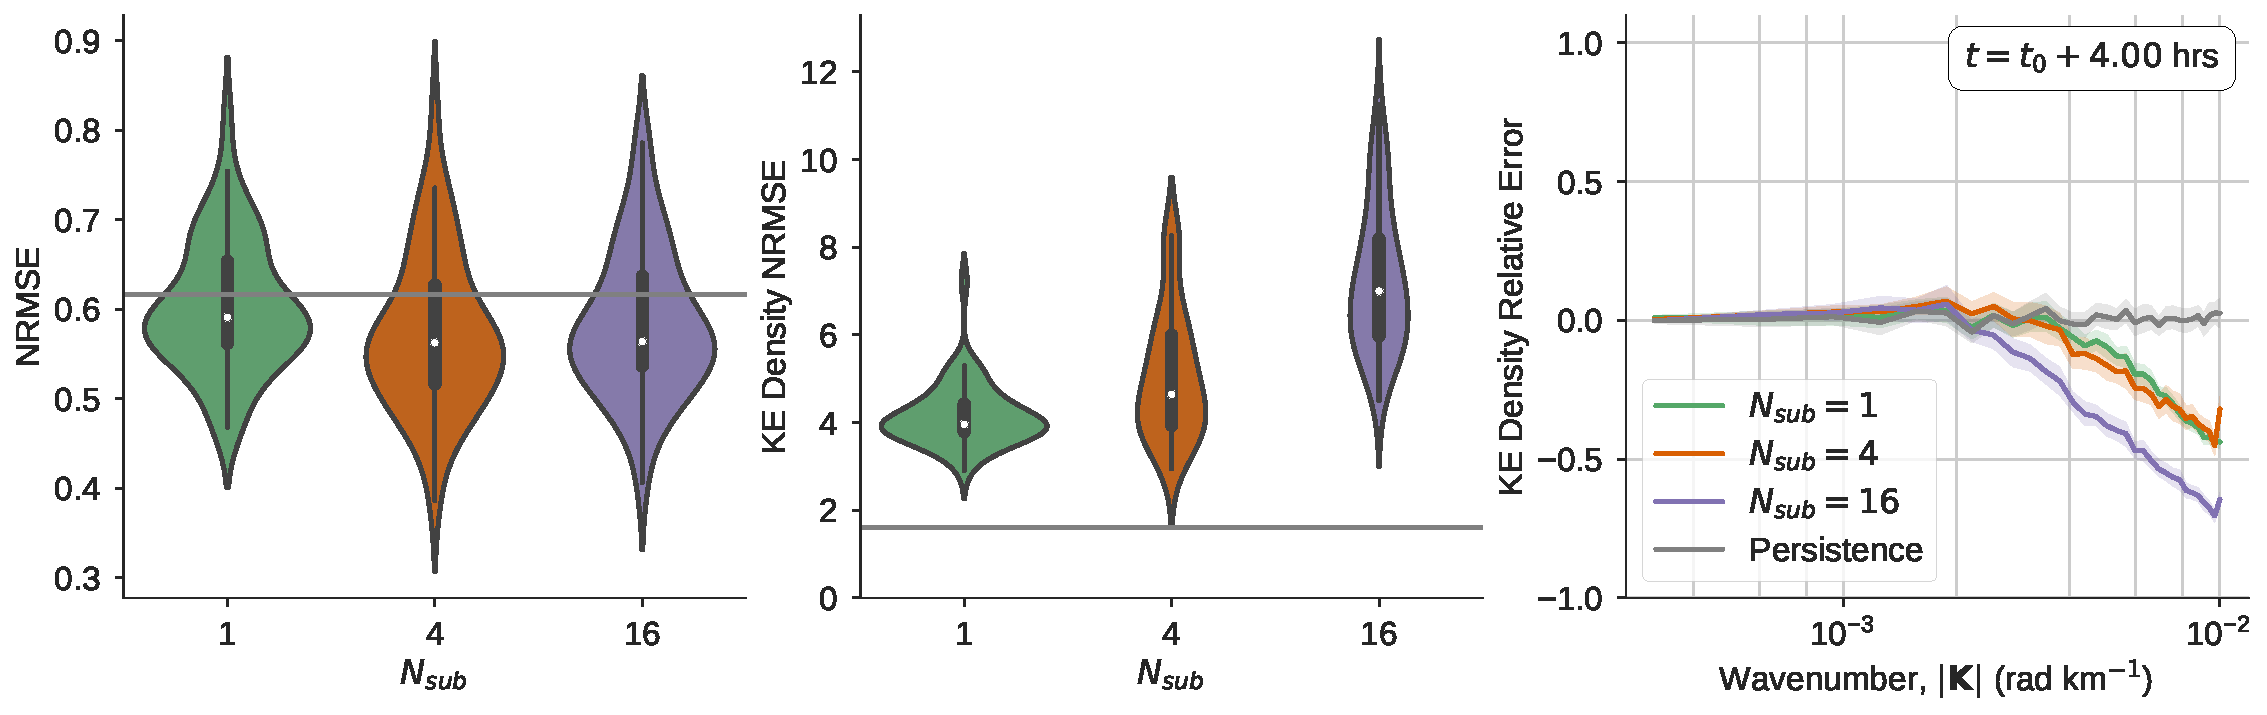
\includegraphics[width=\textwidth]{../figures/rc_all_gamma0.1.pdf}
    \caption{Quantitative comparison of ESN predictions, showing
        NRMSE (a), KE\_NRMSE (b), and KE relative error (c), exactly as in
        \cref{fig:rc_quantiative_nsub01}, except here $\gamma=10^{-1}$ is fixed,
        and the temporal subsampling factor is varied: $\nsub=\{1,4,16\}$.
    }
    \label{fig:rc_quantiative_gamma0.1}
\end{figure}

Interestingly, there is little difference between NRMSE obtained by the ESNs at
different $\nsub$ values.
Additionally, \cref{fig:rc_quantiative_gamma0.0} shows that there is little
difference in NRMSE even when $\gamma=0$, i.e., when NRMSE is the only criterion
for parameter selection.
Therefore, if the goal is to simply produce a prediction with minimal RMSE over a
12~hour window, then it is beneficial to subsample the data in time because of
the improvements in computational efficiency.
However, if the goal is to represent all spatial scales in the data as well as
possible, then NRMSE alone is not a good criterion for model selection.
This assertion is corroborated by the discussion in \cref{subsec:esn-ego}, and
with the fact that when $\gamma=0$ there is little difference in KE error
no matter how the data are subset, even though this difference is stark when
KE density is more appropriately prioritized.

\begin{figure}
    \centering
    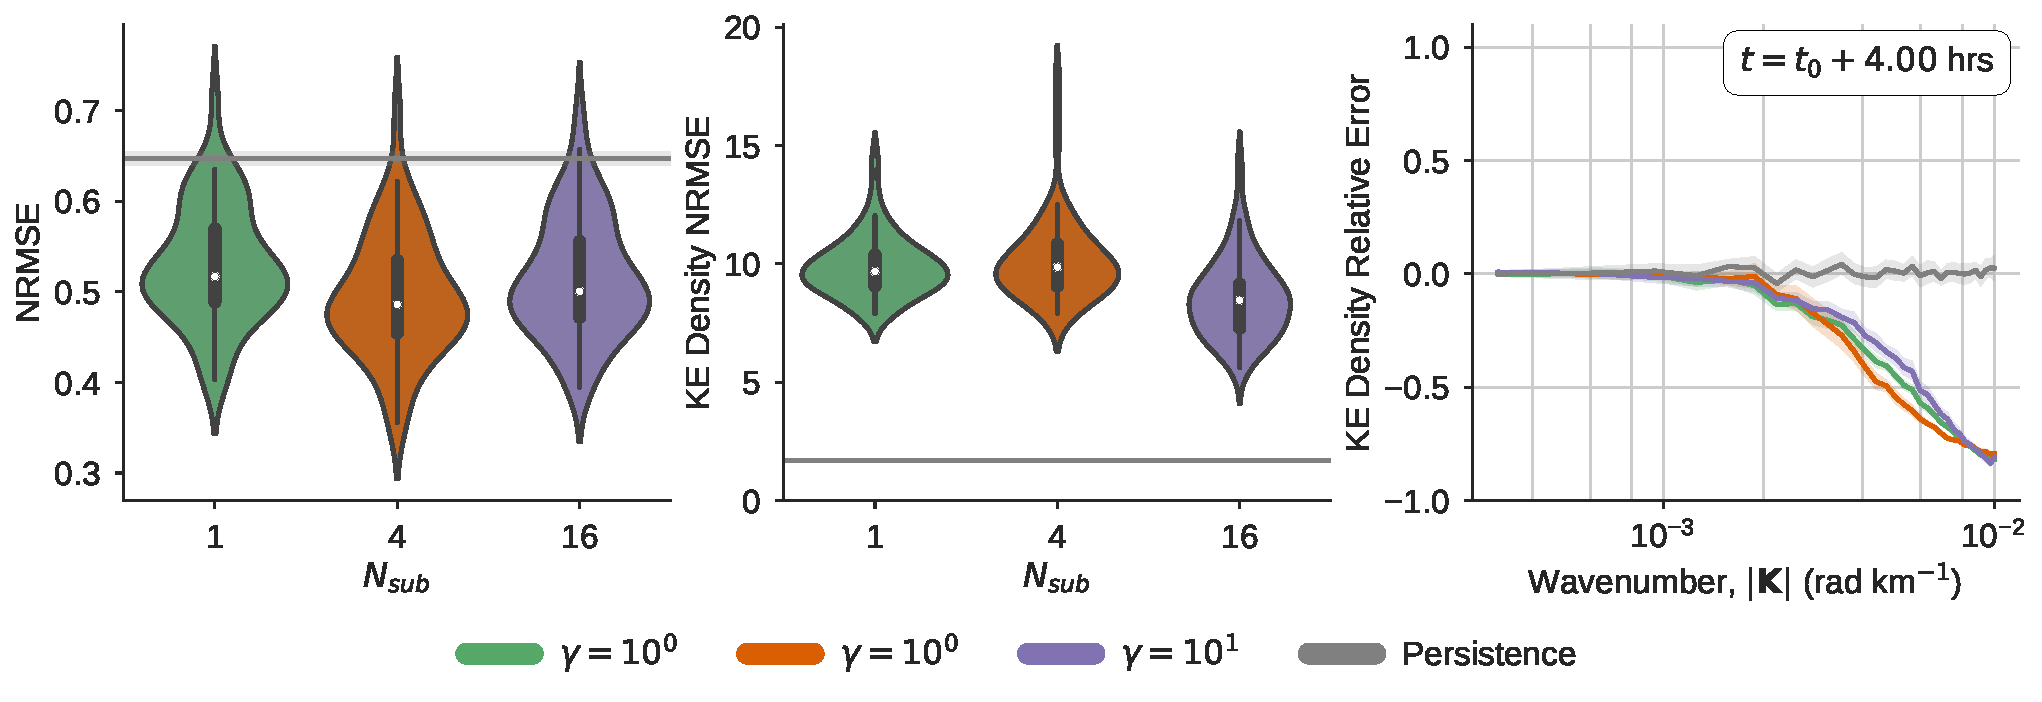
\includegraphics[width=\textwidth]{../figures/rc_all_gamma0.0.pdf}
    \caption{Same as \cref{fig:rc_quantiative_gamma0.1}, except here $\gamma=0$.}
    \label{fig:rc_quantiative_gamma0.0}
\end{figure}

\subsection{Impact of reservoir size}
\label{subsec:esn-size}

The size of the reservoir, $\nhidden$, determines the
memory capacity available to the ESN
\citep{jaeger_echo_2001,lukosevicius_practical_2012}.
For systems with high dimensional input signals, it is crucial to use a ``large
enough'' reservoir to afford the memory capacity necessary for accurate
predictions \citep{hermans_memory_2010}.
In all the preceding sections we fixed $\nhidden=6,000$ at each local group,
where for reference each local group has an input dimension of
$\ninputstate=200$ and an output dimension of $\nstate=128$.
Here, we briefly address the effect of doubling the reservoir size,
while keeping the input and output dimensions constant, in order to test how
sensitive our conclusions are on this crucial hyperparameter.
Due to the computational expense of the parameter optimization discussed in
\cref{subsec:esn-ego}, we only perform this experiment for $\nsub=16$.

The impact of doubling $\nhidden$ on prediction skill is shown in
\cref{fig:esn-size}, where for the sake of brevity we only show results for the
case when $\gamma=0.1$ in \cref{eq:macro-cost}.
Panel (a) shows that the larger reservoir actually reduces the NRMSE slightly.
However, panels (b) and (c) show that this reduction is due to the improved
representation of KE density.
The improvement in KE\_NRMSE is nearly proportional to the improvement achieved by increasing
the temporal resolution of the data.
That is, doubling the reservoir size improves the average KE\_NRMSE by 14\%,
while increasing the temporal resolution of the data by a factor of 4 improves
the KE\_NRMSE by 30\%.

\begin{figure}
    \centering
    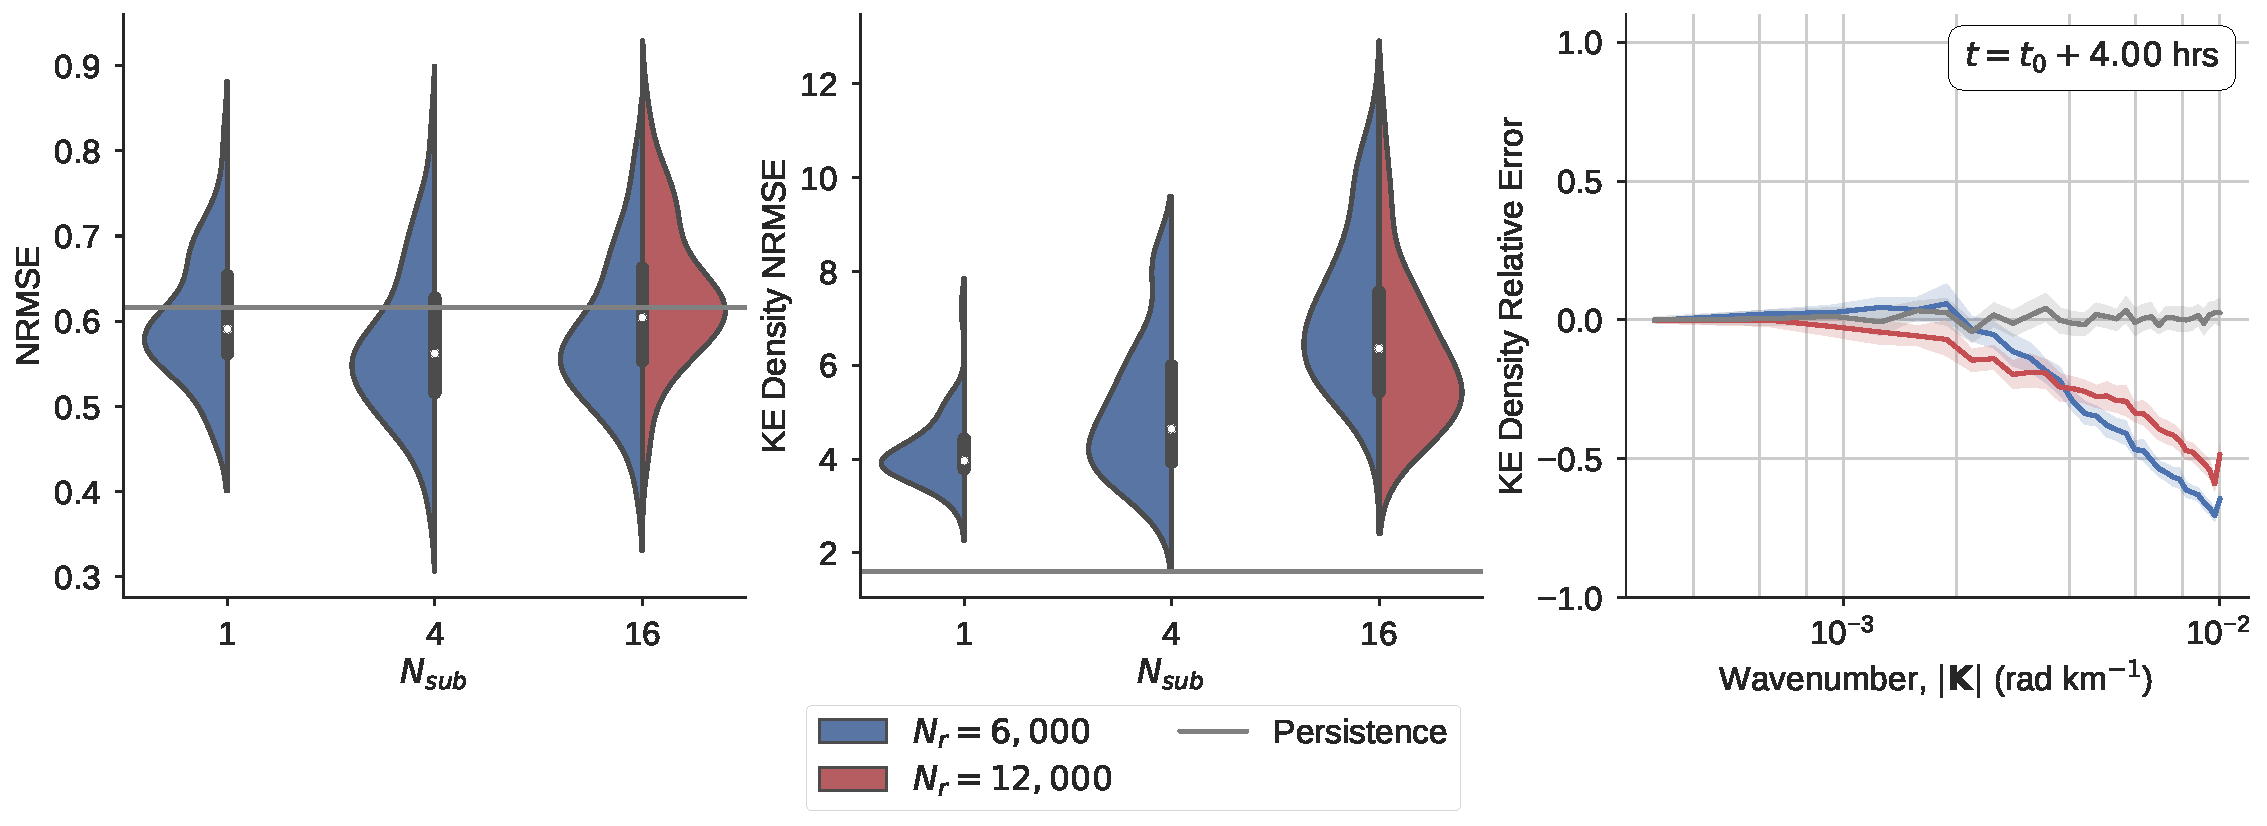
\includegraphics[width=\textwidth]{../figures/rc_reservoir_size.pdf}
    \caption{The impact of doubling the reservoir size from $\nhidden=6,000$ to
        $\nhidden=12,000$ on NRMSE (a), KE\_NRMSE (b), and KE relative error (c).
        Here $\gamma=0.1$.
    }
    \label{fig:esn-size}
\end{figure}


\section{Discussion}
\label{sec:discussion}

\begin{itemize}
    \item Does it matter for error covariances?
    \item Note that this has a sort of reverse CFL condition compared to
        traditional numerical modeling
\end{itemize}


NVAR future work
\begin{itemize}
    \item Multistep training like in \citep{weyn_improving_2020}
    \item Include $\psi$ streamfunction
\end{itemize}

RC Future work
\begin{itemize}
    \item reduce reservoir size with POD or controllability matrix or
        autoencoder
    \item what about multi scale papers
    \item what about CNN ESN
\end{itemize}



\appendix
\section{Matrix and Data Normalization for Reservoir Computing}
\label{sec:new_methods}

Here we describe several aspects of our RC implementation that are
unique with respect to previous works.
Additionally we provide some empirical justification for these choices, using
the Lorenz96 model as a testbed \citep{lorenz_predictability_1996}, see
Appendix \cref{subsec:lorenz96} for a description of the datasets generated for these
tests.

Our testing framework follows the general procedure laid out
by \citet{platt_systematic_2022} to evaluate the architecture choices.
For each design choice, we compute the Valid Prediction Time (VPT) of
an RC model over 100 randomly chosen initial conditions from a test dataset.
VPT is computed as
\begin{linenomath*}\begin{equation*}
    \begin{aligned}
        \text{VPT} &= \argmin_{n} \left\{ \text{NRMSE}(n) > \epsilon \right\} \\
        \text{NRMSE}(n) &= \sqrt{\dfrac{1}{\nstate}\sum_{i=1}^{\nstate}\left(
            \dfrac{\hat{v}_i(n) - v_i(n)}{SD_i}
            \right)^2
        } \, ,
    \end{aligned}
\end{equation*}\end{linenomath*}
where $n$ is a time index, $SD_i$ is the temporal standard deviation of the $i$-th dimension,
computed from the training data, and $\epsilon=0.2$.
To eliminate the dependence of the results on the randomly chosen adjacency and
input matrices, we repeat the process for 10 different adjacency and input
matrix pairs, initialized with different random number generator seeds.
In total, we compare each design choice with a VPT distribution from 1,000 test samples.
We note that we optimize the RC parameters listed in
\cref{eq:rc-hyperparameters} for each design choice and each random matrix pair,
following the procedure laid out in \cref{sec:optim}.
Of course, these tests are insufficient to definitively prove that these choices
will translate perfectly to the SQG system.
However, we consider this to be a bare minimum test that will catch downright bad
design choices, while saving the computing resources necessary to train an
emulator for larger problems.


\subsection{Input Matrix Scaling}

Typically, $\inputmatrix$ is filled with entries
\begin{linenomath*}\begin{equation*}
    \hat{w}_{i,j} \sim \mathcal{U}(-\sigma,\sigma) \qquad
    i = [1, 2, ..., \nhidden], j=[1,2, ..., \ninputstate] \,
\end{equation*}\end{linenomath*}
where $\sigma$ is a hyperparameter that determines the bounds of the uniform
distribution.
Here we found it to be advantageous to normalize the input matrix by the
largest singular value.
That is, we first compute $\hat{\mathbf{W}}_\text{input}$, with elements
\begin{linenomath*}\begin{equation*}
    \hat{w}_{i,j} \sim \mathcal{U}(-1,1) \qquad
    i = [1, 2, ..., \nhidden], j=[1,2, ..., \ninputstate] \, .
\end{equation*}\end{linenomath*}
Then, we set $\inputmatrix$ as
\begin{linenomath*}\begin{equation*}
    \inputmatrix \coloneqq
    \dfrac{\sigma}{\sigma_{max}\left(\hat{\mathbf{W}}_\text{in}\right)}
    \hat{\mathbf{W}}_\text{in} \,
\end{equation*}\end{linenomath*}
where $\sigma_{max}\left(\cdot\right)$ is the largest singular value, and
the hyperparameter $\sigma$ is the desired largest singular value of
$\inputmatrix$.

Our motivation for using this type of normalization is that we found it
necessary to use very wide hyperparameter optimization bounds for $\sigma$ when
using the standard input scaling strategy.
By first normalizing the matrix by the largest singular value compensates for the fact that
the amplitude of the contributions to the reservoir, i.e., the elements of the
vector
\begin{linenomath*}\begin{equation*}
    \mathbf{p} = \inputmatrix \inputstate =
    \begin{pmatrix}
        \mathbf{w}_1^T\inputstate \\
        \mathbf{w}_2^T\inputstate \\
        \vdots \\
        \mathbf{w}_{\nhidden}^T\inputstate
    \end{pmatrix}
\end{equation*}\end{linenomath*}
grow with $\ninputstate$. \todo{this would be the place to talk about variance}
By controlling for this growth, we were able to reduce the optimization search
space and achieve more consistent prediction skill with fewer iterations.

Additionally, we found empirical evidence to suggest that this normalization is
advantageous even for small systems.
\cref{fig:simple-normalization} shows the VPT achieved with
the 20-Dimensional Lorenz96 system (\cref{subsec:lorenz96}), using a variety of
normalization strategies for the input and adjacency matrices.
In \cref{fig:simple-normalization}, the two schemes used for the input matrix
are (1) no normalization (indicated by $c W_{in}$ in
\cref{fig:simple-normalization}) and
(2) normalization by the largest singular vector (indicated by
$\sigma_{max}(W_{in})$).
For a variety of reservoir sizes ($\nhidden$), we found that using the largest
singular vector often performed better, usually by about 0.5~MTU.

\begin{figure}
    \centering
    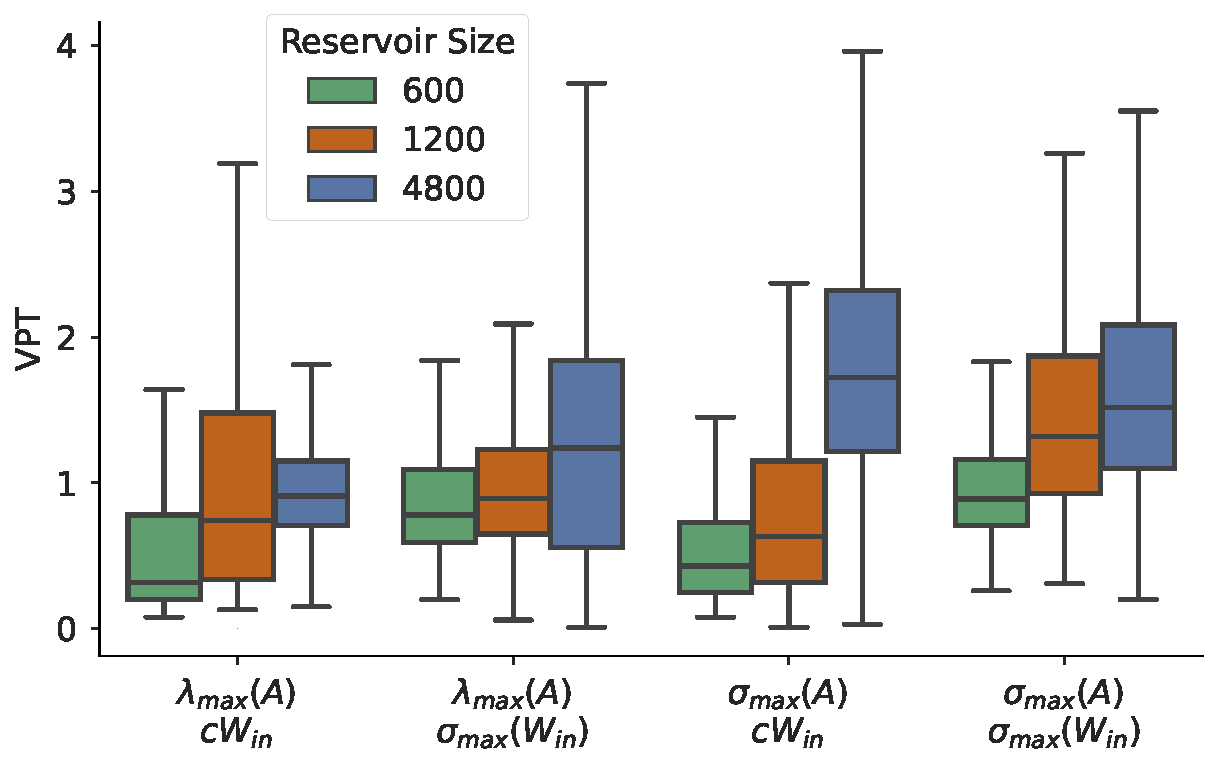
\includegraphics[width=.8\textwidth]{../figures/matrix_normalization.pdf}
    \caption{Valid Prediction Time (VPT) with reservoir computing, using
        different normalization strategies for the adjacency and input matrices,
        $\adjacency$ and $\inputmatrix$. The normalization used for each matrix
        is indicated as follows:
        $\lambda_{max}(\cdot)$ refers to the largest eigenvalue (i.e.,
        spectral radius),
        $\sigma_{max}(\cdot)$ refers to the largest singular value (i.e.,
        induced 2 norm),
        while $c$ implies that no normalization was used.
        The results are computed with the 20D Lorenz96 system, described in
        \cref{subsec:lorenz96}.
        The boxplots indicate prediction skill from 10 different adjacency and
        input matrices (achieved by changing the random number generator seed),
        with 100 initial conditions randomly sampled from the test dataset for
        each set of matrices.
        The hyperparameters were optimized for each unique matrix pair.
        Color indicates the size of the reservoir used.
    }
    \label{fig:simple-normalization}
\end{figure}

\subsection{Adjacency Matrix Scaling}

Typically, the reservoir adjacency matrix is normalized to achieve a desired
spectral radius.
That is, the matrix $\hat{\adjacency}$ is generated with elements
$\hat{a}_{i,j} \sim \mathcal{U}(-1,1)$, where $i,j$ are random indices in order
to satisfy the desired sparsity of the matrix (all other elements are 0).
Then, the $\adjacency$ is set as
\begin{linenomath*}\begin{equation*}
    \adjacency \coloneqq
    \dfrac{\spectralradius}{\lambda_{max}\left(\hat{\adjacency}\right)}
    \hat{\adjacency} \, ,
\end{equation*}\end{linenomath*}
where $\lambda_{max}\left(\cdot\right)$ is the spectral radius, and $\spectralradius$
scales the matrix to achieve the desired spectral radius.
A common guideline is to set $\spectralradius \simeq 1$, as it is hypothesized
that this puts the reservoir on the ``edge of stability'' so that it performs
well in emulating nonlinear systems \red{CITE}.
However, as originally described by \citet{jaeger_echo_2001},
using the spectral radius is only a necessary, but insufficient means to satisfy
the Echo State Property \red{DEFINE THIS}.
On the other hand, using the largest singular value is a sufficient condition
for satisfying the echo state property.

In our experimentation, we have found a slight benefit from using the largest
singular value to normalize the adjacency matrix.
\cref{fig:simple-normalization} shows that, for fixed input matrix
normalization, using the largest singular value rather than spectral radius
achieves similar and up to $\sim0.3$ longer valid predictions.
While the improvement is subtle, we note that using the largest singular value
has the following practical benefit for our python-based implementation:
the singular values can be computed directly on a Graphical Processing Unit
using CuPy \red{CITE CUPY}, while a general, non-symmetric eigenvalue
decomposition is not readily available.

\subsection{Data Normalization}
\label{subsec:data_normalization}

A key aspect in machine learning is normalizing input data before passing it to
the model.
Experiments from \citet{platt_systematic_2022} showed, however, that the
standard approach to normalizing data
be detrimental to prediction skill.
By ``standard  approach'', we mean
\begin{linenomath*}\begin{equation*}
    v_i(n) = \dfrac{v_i(n) - \bar{v}_i}{SD_i} \qquad i = [1, 2, ...
    \nstate]
\end{equation*}\end{linenomath*}
where $\bar{v}_i, SD_i$ are the mean and standard deviation taken from the
training data for each channel
of input data, indexed by $i$.
The key takeaway from \citet{platt_systematic_2022} is that by using separate
normalization values for each channel, the covarying relationships between the
data are destroyed and so the reservoir cannot learn the true dynamics.
They therefore propose to normalize with the average and range of the data,
computed over the length of the training data and over all channels
\begin{linenomath*}\begin{equation}
    v_i(n) = \dfrac{v_i(n) - \bar{\mathbf{v}}}{\max\mathbf{v} - \min\mathbf{v}}
    \qquad i = [1,2, ... \nstate] \, ,
    \label{eq:maxmin}
\end{equation}\end{linenomath*}
Here, we propose to replace the range in the denominator with the
standard deviation computed over all channels and timesteps in the training
data,
\begin{linenomath*}\begin{equation}
    v_i(n) = \dfrac{v_i(n) - \bar{\mathbf{v}}}{SD}
    \qquad i = [1,2, ... \nstate] \, .
    \label{eq:sdnorm}
\end{equation}\end{linenomath*}

\cref{fig:data-norm} compares the prediction skill when these two normalization
strategies are used.
Using the standard deviation normalization as in \cref{eq:sdnorm} leads to an
average VPT increase by two.
We surmise that this improvement is due to the fact that when the data are
normalized by the full range, then all values are in the range $[-1,1]$.
In this case, once the input is mapped into the hidden space, it is more likely
to lie on the linear regime of the $\tanh(\cdot)$ activation function.
While a large enough input scaling could eliminate this problem, it is
apparently not easily obtained during the hyperparameter optimization.

\begin{figure}
    \centering
    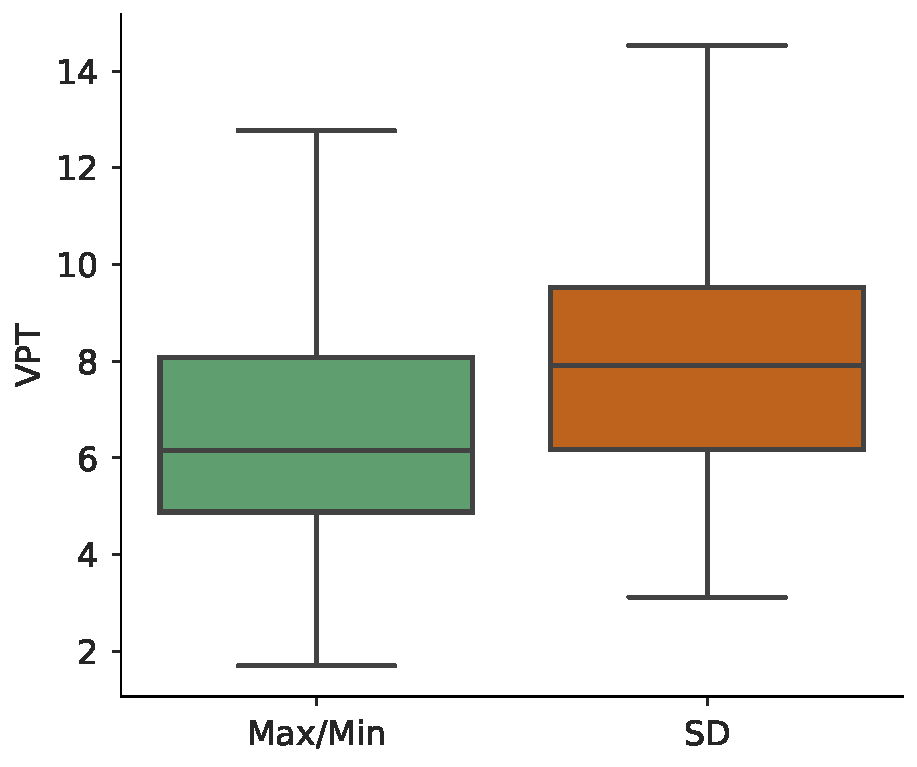
\includegraphics[width=.6\textwidth]{../figures/data-normalization.pdf}
    \caption{Valid Prediction Time (VPT) with reservoir computing, using the
        Max/Min normalization strategy shown in \cref{eq:maxmin} and standard
        deviation (SD)
        normalization strategy as in \cref{eq:sdnorm}.
        The results are computed with the 6D Lorenz96 system, described in
        Appendix \cref{subsec:lorenz96}.
        The boxplots indicate prediction skill from 10 different adjacency and
        input matrices (achieved by changing the random number generator seed),
        with 100 initial conditions randomly sampled from the test dataset for
        each set of matrices.
        The hyperparameters were optimized for each unique matrix pair.
    }
    \label{fig:data-norm}
\end{figure}

\subsection{Lorenz96 Datsets}
\label{subsec:lorenz96}


\red{Description of the L96 dataset...}

\section{Bayesian Optimization for Parameter Selection}
\label{sec:optim}

\red{Talk about parameter optimization here}

\section{Gulf of Mexico Dataset}
\label{sec:gom}



\newpage
\section{Open Research}
AGU requires an Availability Statement for the underlying data needed to understand, evaluate, and build upon the reported research at the time of peer review and publication.

Authors should include an Availability Statement for the software that has a significant impact on the research. Details and templates are in the Availability Statement section of the Data and Software for Authors Guidance: \url{https://www.agu.org/Publish-with-AGU/Publish/Author-Resources/Data-and-Software-for-Authors#availability}

It is important to cite individual datasets in this section and, and they must be included in your bibliography. Please use the type field in your bibtex file to specify the type of data cited. Some options include Dataset, Software, Collection, ComputationalNotebook. Ex:

%%%%%%%%%%%%%%%%%%%%%%%%%%%%%%%%%%%%%%%%%%%%%%%

\acknowledgments

T.A. Smith and S.G. Penny acknowledge support from NOAA grant NA20OAR4600277. S.G. Penny and J.A. Platt acknowledge support from the Office of Naval Research (ONR) grants N00014-19-1-2522 and N00014-20-1-2580. T.-C. Chen is supported by the NOAA Cooperative Agreement with CIRES, NA17OAR4320101.

This section is optional. Include any Acknowledgments here.
The acknowledgments should list:\\
All funding sources related to this work from all authors\\
Any real or perceived financial conflicts of interests for any author\\
Other affiliations for any author that may be perceived as having a conflict of interest with respect to the results of this paper.\\
It is also the appropriate place to thank colleagues and other contributors. AGU does not normally allow dedications.




%% ------------------------------------------------------------------------ %%
%% References and Citations

%%%%%%%%%%%%%%%%%%%%%%%%%%%%%%%%%%%%%%%%%%%%%%%
%
% don't specify bibliographystyle
\bibliography{references}


\end{document}
